% Created 2020-12-06 Sun 13:11
% Intended LaTeX compiler: pdflatex
\documentclass[11pt]{article}
\usepackage[utf8]{inputenc}
\usepackage[T1]{fontenc}
\usepackage{graphicx}
\usepackage{grffile}
\usepackage{longtable}
\usepackage{wrapfig}
\usepackage{rotating}
\usepackage[normalem]{ulem}
\usepackage{amsmath}
\usepackage{textcomp}
\usepackage{amssymb}
\usepackage{capt-of}
\usepackage{hyperref}
\usepackage{minted}
\author{Dustin Leatherman}
\date{\today}
\title{Bayesian Statistics}
\hypersetup{
 pdfauthor={Dustin Leatherman},
 pdftitle={Bayesian Statistics},
 pdfkeywords={},
 pdfsubject={},
 pdfcreator={Emacs 26.1 (Org mode 9.5)}, 
 pdflang={English}}
\begin{document}

\maketitle
\tableofcontents


\section{Intro (2020/09/10)}
\label{sec:orge420207}

\subsection{Motivating Example}
\label{sec:orga538e3f}
There are two students: Student A and Student B, along with an instructor.
A secretly writes down a number (1,..,10) then mentally calls heads or tails.

\begin{enumerate}
\item The instructor flips a coin
\item If heads, A honestly tells B if the number is even or odd.
\item If A guesses H/T correctly, A tells B if their number is even or odd.
Otherwise, they lie.
\item B will guess if the number is odd or even

Let \(\theta\) be the probability that B correctly guesses even or odd.
\end{enumerate}

\begin{quote}
The class (and myself) initially agreed without much discussion that 0.5 is the
obvious answer. Upon further thinking on this, the probabilities breakdown in
such way:

(2): 0.5
(3): 0.5
(4): ?

The initial logic is that its a 50/50 chance since there are two choices but
there is an X-factor here with number 4. A few questions worth asking:
\begin{enumerate}
\item Does B know the rules upfront? As in, are they
\end{enumerate}
aware that A may or may not lie?
\begin{enumerate}
\item Does B see the result of the coin flip?
\item Is this done virtually or in person?
\end{enumerate}

If the answer is no for 1 and 2, then 0.5 is a logical choice because they'd
be guessing without much foreknowledge.

If the answer is yes for 1 and 2, then B is in on the ``game'' and can make a more
educated guess. If A or the professor has a ``tell'', then that could provide
information. Reading body language may also provide some information to B on the
veracity of A's claim.

I would argue that \(\theta\) would be > 0.5 \emph{if} A and B know each other well
enough. Which is really a great example of Bayesian vs Frequentist view points.
\end{quote}


\subsection{Frequentist Approach}
\label{sec:org5e6425a}

Quantifies uncertainty in terms of repeating the process that generated the data
many times.

\subsubsection{Properties}
\label{sec:org72cb496}
\begin{itemize}
\item The parameters \(\theta\) are fixed, unknown, and a constant.
\item The sample (data) Y are random
\item All prob. statements would be made about the randomness in the data.
\item 
\end{itemize}

A statistic \(\hat \theta = Y / n\) is a statistic and is an estimator of the
population proportion \(\theta\)

The distribution of \(\hat \theta\) from repeated sampling is the \emph{sample distribution}.
\subsubsection{Things a Frequentist would never say}
\label{sec:org8393a2b}
\begin{itemize}
\item \(P(\theta > 0) = 0.6\) because \(\theta\) is not a random variable
\item The distribution of \(\theta\) is Normal(4.2,1.2)
\item The probability that the true proportion is in the interval (0.4, 0.5) is
0.95.
\item The probability that the null hypothesis is true is 0.03.
\end{itemize}


\subsection{Bayesian Approach}
\label{sec:orgf6be91e}

Expresses uncertainty about \(\theta\) using probability distributions. \(\theta\)
is still fixed and unknown.

Distribution \emph{before} observing the data is the \textbf{prior distribution}. e.g.
\(P(\theta > 0.5) = 0.6\). This is subjective since people may have different priors.

Hopefully, Uncertainty about \(\theta\) is reduced after observing the data.

Bayesian Interpretations differ from \emph{Frequentist} Interpretations.

Uncertainty distribution of \(\theta\) after observing the data is the \textbf{posterior
distribution}.

\textbf{Bayes Theorem} for updating the prior

\begin{equation}
\begin{split}
f(\theta | Y) = \frac{f(Y | \theta) f(\theta)}{f(Y)}
\end{split}
\end{equation}

Described in words: Posterior \(\propto\) Likelihood \(\times\) Prior

\begin{quote}
\(f(\theta | Y)\) is the posterior distribution.

Given that I have seen some data, what am I seeing now?
\end{quote}

A key difference between Bayesian and frequentist statistics is that all
inference is conditional on the single data set we observed (Y).



\subsubsection{Likelihood Function}
\label{sec:org31e794b}

Distribution of the observed data given the parameters. This is the Same
function used in a maximum likelihood analysis.

\begin{quote}
When prior information is weak, Bayesian and Maximum Likelihood Estimates are similar.
\end{quote}

\subsubsection{Priors}
\label{sec:org84f5547}

Say we observed Y = 60 successes in n = 100 trials and \(\theta \in [0,1]\) is the
true probability of success.

Want to select a prior that has a domain of [0, 1]

If there is no relevant prior information, we might use \(\theta \sim Uni(0,1)\).
This is called an \emph{uninformative prior}. aka a ``best guess''.

\begin{enumerate}
\item Beta
\label{sec:org2dcadd7}

Beta distributions are a common prior for parameters between 0 and 1.

If \(\theta \sim Beta(a, b)\), then the posterior is

$$
\theta | Y \sim Beta(Y + a, n - Y + b)
$$


\(Beta(1,1) == Uni(0,1)\)

\item Gamma
\label{sec:orga22dfa1}
Popular distribution for \(\sigma\) (population standard deviation)
\end{enumerate}

\subsubsection{Posteriors}
\label{sec:org168508e}

The likelihood function \(Y | \theta \sim Bin(n, \theta)\)

The Uniform prior is \(\theta \sim Uni(0, 1)\)

The posterior is then \(\theta | Y \sim Beta(Y + 1, n - Y + 1)\)

\subsubsection{Advantages}
\label{sec:org6ffe0b2}
\begin{itemize}
\item Bayesian concepts (posterior probability of the null hypothesis) are arguably
easier to interpret than the frequentist ideas (p-value.)
\item Can incorporate scientific knowledge via the prior.
\begin{itemize}
\item Even a Small amount of prior information can add stability.
\end{itemize}
\item Excellent at quantifying uncertainty in complex problems.
\item Provides a framework to incorporate data/information from multiple sources.
\end{itemize}

\subsubsection{Disadvantages}
\label{sec:org55093de}
\begin{itemize}
\item Less common/familiar
\item Picking a prior is subjective (though there are objective priors)
\item Procedures with frequentist properties are desirable.
\item Computing can be slow for hard problems
\item Non parametric methods are challenging
\end{itemize}

\subsection{Review}
\label{sec:org7b10b4e}

\begin{quote}
Only the interesting parts are placed here. See the rest of this repo for deeper
dives on other concepts.
\end{quote}

\subsubsection{Probability}
\label{sec:orgc1af0b5}
Objective (associated with Frequentist)
\begin{itemize}
\item \(P(X = x)\) is a mathematical statement
\item If we repeatedly sampled X, the value that the proportion of draws equal to x
converges is defined as \(P(X = x)\)
\end{itemize}

Subjective (associated with Bayesian)
\begin{itemize}
\item \(P(X = x)\) represents an individual's degree of belief
\item Often quantified as the amount an individual would be willing to wager that X
will be x.
\end{itemize}

A Bayesian Analysis uses both of these concepts.

\subsubsection{Uncertainty}
\label{sec:orgf0d4dca}

Aleatoric (def: indeterminate) uncertainty (likelihood)
\begin{itemize}
\item Uncontrollable randomness in the experiment
\end{itemize}

Epimestic (def: involving knowledge) uncertainty (prior/posterior)
\begin{itemize}
\item Uncertainty about a quantity that could be theoretically
\end{itemize}

A Bayesian Analysis uses both of these concepts

\subsubsection{Probability vs Statistics}
\label{sec:orgd30d67c}

\begin{quote}
The common sense, I like the way this is phrased.
\end{quote}

Probability is the forward problems
\begin{itemize}
\item We assume we know how the data are being generated and computer the
probability of events.

For example, what is the probability of flipping 5 straight heads if the coins
are fair?
\end{itemize}

Statistics is the inverse problem
\begin{itemize}
\item We use data to learn about the data-generating mechanism

For example, if we flipped five straight heads, can we conclude the coin is
biased?
\end{itemize}
\section{Probability \& Introduction to Bayes (2020/09/17)}
\label{sec:orge0f6307}


if x and y are independent, then the following is true

$$
f(x | y) = \frac{f(x, y)}{f_Y (y)} = \frac{f_X(x) f_Y (y)}{f_Y (y)} = f_X (x)
$$


Cannot use \(f(x,y)\) as PMF because \(\sum_{1}^{Y} f(x,y) = f(x) \neq 1\). Need to
scale by marginal probability in order to sum to 1 and thus be a proper PMF/PDF.

\begin{center}
\begin{tabular}{lrrrrrr}
 & 1 & 2 & 3 & 4 & 5 & Total [p(y)]\\
\hline
US & .0972 & .0903 & .0694 & .0069 & .0069 & .2708\\
Not US & .3194 & .1319 & .1389 & .1181 & .0208 & .7292\\
Total [p(x)] & .4167 & .2222 & .2083 & .1250 & .0278 & 1\\
\end{tabular}
\end{center}

show that x and y are dependent

\(P(x = 1) = 0.4167\)

\(P(y = 1) = 0.2708\)

\(P(x = 1) \times P(y = 1) = 0.4167 (0.2708) = 0.1128\)

\(P(x = 1, y = 1) = 0.0972 \neq 0.1128\) so dependent!

\subsection{Calculating the Posterior Analytically}
\label{sec:org3974354}

\subsubsection{Using an Arbitrary PDF}
\label{sec:org085b91f}

\begin{enumerate}
\item Find Joint Probability (f(x,y))
\end{enumerate}

\begin{equation}
\begin{split}
P(x > 7, y > 40) = & \int_{7}^{10} \int_{40}^{50} \ 0.26 exp(- |x - 7| - |y - 40|) \ dx \ dy\\
    = & 0.26 \ \int_{7}^{10} \int_{40}^{50} exp(- x + 7 - y + 40) \ dx \ dy \label{eq:21a} \ (\text{Since only interested in positive values})\\
    = & 0.26 \ \int_{7}^{10} \int_{40}^{50} exp(- (x - 7) \ exp( - (y - 40)) \ dx \ dy\\
    = & 0.26 \ \int_{7}^{10} \int_{0}^{10} exp(- (x - 7) \ exp(-u) \ dx \ du\\
    = & 0.26 \ \int_{7}^{10} \int_{0}^{10} exp(- (x - 7) \ [- exp(-u)]_0^{10} \ dx \ du\\
    = & 0.26 (1 - e^{-10}) \ \int_{7}^{10} exp(- (x - 7) dx\\
    = & 0.26 (1 - e^{-10}) (1 - e^{-3}) \approx 0.247
\end{split}
\end{equation}

\begin{enumerate}
\item Find Marginal Probability over the Data \(f_X(x)\)
\end{enumerate}

\begin{equation}
\begin{split}
f_X(x) = & \int_{20}^{50} 0.26 + e^{- |x - 7| - |y - 40|} dy\\
    = & 0.26 e ^{-|x - 7|} \int_{20}^{50} e^{- |y - 40|} dy\\
    = & 0.26 e ^{-|x - 7|} [\int_{20}^{40} e^{- (40 - y)} dy +  \int_{40}^{50} e^{- (y - 40)} dy]\\
    = & 0.26 e ^{-|x - 7|} [\int_{20}^{0} - e^{-u} du +  \int_{0}^{10} e^{- u} du]\\
    = & 0.26 e ^{-|x - 7|} [1 - e^{-20} + 1 - e^{-10} \approx 2 ] \\
    = & 0.52 e ^{- |x - 7|} \ \forall \ x \leq x \leq 10
\end{split}
\end{equation}

\begin{enumerate}
\item Calculate Conditional Probability
\end{enumerate}

$$
f(y | x) = \frac{f(x, y)}{f_X (x)} = \frac{1}{2} e^{- |y - 40|}
$$

\begin{quote}
If integrating over an absolute value, break up the integral into two integrals:
the first over the negative domain of the integration, the second over the
positive domain.
\end{quote}

\subsubsection{Using Normal Distribution}
\label{sec:org1a7d627}

\begin{enumerate}
\item Find Marginal Probability
\end{enumerate}

\begin{equation}
\begin{split}
f(x) = & \int_{- \infty}^{\infty} \frac{1}{2 \pi \sqrt{1 - \rho^2}} \ exp(- \frac{x^2 + y^2 - 2 \rho x y}{2 (1 - \rho^2)}) \ dy\\
= & \frac{1}{2 \pi \sqrt{1 - \rho^2}} e^{-x^2 / 2(1 - \rho^2)} \ \int_{- \infty}^{\infty} \frac{1}{\sqrt{2 \pi}} exp(- \frac{y^2 - 2 \rho x y}{2 (1 - \rho^2)}) \ dy \label{eq:2b1} \ \text{(Move x's out of integral. Arrange terms so it looks like a Normal Distribution.)}\\
= & \frac{1}{\sqrt{2 \pi} \sqrt{1 - \rho^2}} e^{-x^2 / 2(1 - \rho^2)} \ \int_{- \infty}^{\infty} \frac{\sqrt{1 - \rho^2}}{\sqrt{2 \pi (1 - \rho^2)}} exp(- \frac{y^2 - 2 \rho x y + \rho^2 x^2 - (\rho x)^2}{2 (1 - \rho^2)}) \ dy\\
= & \frac{1 \ \sqrt{1 - \rho^2}}{\sqrt{2 \pi} \sqrt{1 - \rho^2}} e^{-x^2 / 2(1 - \rho^2)} \ e^{\frac{\rho x^2}{2 (1 - \rho^2)}} \ \int_{- \infty}^{\infty} \frac{1}{\sqrt{2 \pi (1 - \rho^2)}} exp(- \frac{(y - \rho x)^2}{2 (1 - \rho^2)}) \ dy, \label{eq:2b2} \ \mathnormal{N(\rho x, 1 - \rho^2)}\\
= & \frac{1}{\sqrt{2 \pi}} e^{-0.5 \ \frac{x^2 - \rho^2 x^2}{1 - \rho^2}}\\
= & \frac{1}{\sqrt{2 \pi}} e^{-0.5 x^2}, \label{eq:2b3} \mathnormal{X \sim N(0, 1)}\\
\end{split}
\end{equation}

\begin{enumerate}
\item Assume Joint Normal PDF

\item Find Conditional probability
\end{enumerate}

\begin{equation}
\begin{split}
f(y | x) = & \frac{f(x,y)}{f_X (x)}\\
    = & \frac{\frac{1}{2 \pi \sqrt{1 - \rho^2}} exp(- \frac{x^2 + y^2 - 2 \rho x y}{2 (1 - \rho^2)})}{\frac{1}{\sqrt{2 \pi}} \ exp(- \frac{x^2}{2})}\\
    = & \frac{1}{\sqrt{2 \pi} \sqrt{1 - \rho^2}} \ exp(- \frac{x^2 + y^2 - 2 \rho x y}{2 (1 - \rho^2)} + \frac{x^2}{2})\\
    = & \frac{1}{\sqrt{2 \pi} \sqrt{1 - \rho^2}} \ exp(- \frac{1}{2} [\frac{x^2 + y^2 - 2 \rho x y}{1 - \rho^2} - x^2])\\
    = & \frac{1}{\sqrt{2 \pi} \sqrt{1 - \rho^2}} \ exp(- \frac{1}{2} [\frac{x^2 + y^2 - 2 \rho x y - (1 - \rho^2) x^2}{1 - \rho^2}])\\
    = & \frac{1}{\sqrt{2 \pi} \sqrt{1 - \rho^2}} \ exp(- \frac{1}{2} [\frac{y^2 - 2 \rho x y - \rho^2 x^2}{1 - \rho^2}])\\
    = & \frac{1}{\sqrt{2 \pi} \sqrt{1 - \rho^2}} \ exp(- \frac{1}{2} [\frac{(y - \rho x)^2}{1 - \rho^2}]), \ \label{eq:2bd} y|x \sim N(\rho x, 1 - \rho^2)
\end{split}
\end{equation}

\subsection{Bayes Theorem}
\label{sec:orga2f1249}

$$
P(\theta | y) = \frac{P(y | \theta) P (\theta)}{P(y)}
$$

How do you know you are using Bayes Rule?

Given \(P(y | \theta)\), want to find \(P(\theta | y)\)


\begin{itemize}
\item Bayesians quantify uncertainty about fixed but unknown parameters by treating
\end{itemize}
them as random variables.
\begin{itemize}
\item This requires that we set a prior distribution \(\pi(\theta)\) to summarize
uncertainty before observing the data.
\item The distribution of the observed data given the model parameters is the
\emph{likelihood function}, \(f(Y | \theta)\)
\begin{itemize}
\item The likelihood function is the most important piece of a Bayesian Analysis
because it links the data and the parameters.
\end{itemize}
\end{itemize}

\subsection{Bayesian Learning}
\label{sec:org47fff9f}

The posterior distribution \(P(\theta | Y)\) summarizes uncertainty about the
parameters given the prior and data.

Reduction in uncertainty from prior to posterior represents \textbf{Bayesian Learning}

Bayes Theorem (again):

$$
P(\theta | Y) = \frac{f(Y | \theta) \pi (\theta)}{m(Y)}
$$

\(m(Y) = \int F(Y | \theta) \pi (\theta) d \theta\): marginal distribution of the
data and can usually be ignored.

\subsection{Subjectivity}
\label{sec:org65a5889}

Choosing Likelihood function and a prior distribution are subjective.

If readers disagree with assumptions, findings will be rejected so assumptions
must be justified theoretically and empirically.
\section{Summarizing a Posterior Distribution (2020/09/24)}
\label{sec:org661384a}

\subsection{SIR Model}
\label{sec:orge2ff6c3}
Susceptible-Infected-Recovered

At time \(t\) , \(S_t + I_t + R_t = N\) where N is the population.

States evolved according to the following differential equations

\begin{equation}
\begin{split}
\frac{d S_t}{d t} = & -\beta \frac{S-t I_t}{N}\\
\frac{d I_t}{d t} = & \beta \frac{S_t I_t}{N} - \Gamma I_t
\end{split}
\end{equation}

\(\beta\): Controls rate of new infections

\(\Gamma\): Controls recovery rate

We will use a discrete approx to these curves with hourly time steps.

So? \(dt = \frac{1}{24}\)

\textbf{Goal}: Fit SIR Model for given values of \(\beta\) and \(\Gamma\)

\subsection{Summarize a univariate Posterior with Beta-Binomial}
\label{sec:org8a38165}

Posterior = Likelihood \(\times\) Prior

Say there is a parameter \(\theta\)

Likelihood: \(Y | \theta \sim Bin(N, \theta)\)

Prior: \(\theta \sim Uni(0, 1) \equiv Beta(1,1)\)

Posterior: \(\theta | Y \sim Beta(Y + a, N - y + b)\)

\begin{quote}
Peak of the Posterior is the MLE of the Likelihood function when using an
uninformative prior.
\end{quote}

\subsection{MAP Estimator}
\label{sec:orga417478}

Posterior Mode is call the max a posterioiri (MAP) estimator

\begin{equation}
\begin{split}
\hat \theta = \underset{\theta}{argmax} \ P (\theta | y) = \underset{\theta}{argmax} \ log[f(Y | \theta)] + log[\pi(\theta)]
\end{split}
\end{equation}

if prior is uniform, MAP is MLE assuming \(Y | \theta \sim Bin(\theta, n)\).

\subsection{Uncertainty Measures}
\label{sec:org6dad758}

Posterior Std. Dev. is one measure of uncertainty
\begin{itemize}
\item If approx Gaussian, can use empirical rule
\item Analogous but fundamentally different than std error.
\begin{itemize}
\item Std err is the standard deviation of \(\hat \theta\)'s sampling distribution
\end{itemize}
\end{itemize}

Do not call them call them \textbf{confidence} intervals. Called \textbf{Credible} Intervals
in Bayesian Statistics.

Interval \((l, u)\) is 100(\(1 - \alpha\))\% posterior credible interval if \(P(l < \theta < u | Y) = 1 - \alpha\)

Interpretation: ``Given the data and the prior, the probability that \(\theta\) is
between l and u is 0.95.''

\begin{quote}
Confidence interval interpretation:

With 95\% Confidence, \(\theta\) is between l and u.

A Bayesian Posterior is a distribution for \(\theta | Y\) whereas the sampling
distribution is for \(\hat \theta\). While their expected values both represent
the true mean, the sampling distribution is not a distribution of \(\theta\) hence why ``Confidence'' is used when in the interpretation. The Bayesian Posterior is a distribution of \(\theta\) so the posterior can be used for the interpretation.
\end{quote}

\subsubsection{Credible Sets}
\label{sec:org32a9b3c}

Not unique.

Let \(q_\tau\) be the \(\tau\) quantile of the posterior of the posterior such that
\(P(\theta < q_\tau | Y) = \tau\). Then (\(q_{00}, q_{0.95}\)), (\(q_{0.01},
q_{0.96}\)), etc. are all valid 95\% credible sets.

Equal-Tailed intervals: \((q_{\alpha/2}, q_{1 - \frac{\alpha}{2}})\)

\textbf{Highest posterior density} interval searches for the smallest interval  that
contains the proper probability

\subsection{Hypothesis Tests}
\label{sec:org6223285}

Conducted by computing posterior prob of each hypothesis.

$$
P(\theta < 0.5 | Y) = \int_{0}^{0.5} P(\theta | Y) d \theta
$$

analogous but different than a p-value.

\textbf{p-value}: Assuming the null hypothesis is true, the probability we got X or a
value more extreme is Y.

\textbf{Bayesian Hypothesis Test}: Given the prior and the data, the probability the null
hypothesis is true is Y.

\subsection{Monte Carlo Sampling}
\label{sec:org1e6b5e7}

A useful tool for summarizing a posterior.

In MC sampling, we draw S samples from the posterior;

$$
\theta', ..., \theta^{(s)} \sim P(\theta | Y)
$$

and use these samples to approx the posterior.

\subsubsection{Transformations}
\label{sec:org81e13ee}

MC sampling facilitates studying the \textbf{transformations} of parameters.

For example, the odds corresponding to \(\theta\) are \(\gamma = \frac{\theta}{1 - \theta}\)

\begin{equation}
\begin{split}
\gamma^{(1)} = \frac{\theta^{(1)}}{1 - \theta^{(1)}}, ..., \gamma^{(S)} = \frac{\theta^{(S)}}{1 - \theta^{(S)}}
\end{split}
\end{equation}

How to approximate the posterior mean and variance of \(\gamma\)?

Transform the odds and use the draws to approximate \(\theta\)'s posterior!

\subsection{Summarizing Multivariate Posteriors}
\label{sec:org870d8fc}

Univariate posteriors captured by a simple plot. Not easy or impossible to do
with multivariate posteriors.

Let \(\theta = (\theta_1, ..., \theta_p)\).

Ideally, we reduced to the univariate marginal posteriors. Then the same ideas
for univariate models apply

$$
P(\theta_1 | Y) = \int ... \int P(\theta_1, ..., \theta_p | Y) d \theta_2, ...,
d \theta_p
$$

\begin{quote}
Can use Monte Carlo sampling to estimate these integrals.

Need to confirm the above statement
\end{quote}

\subsection{Bayesian One Sample t-test}
\label{sec:orgc9f34ac}

Likelihood: \(Y_i | \mu, \sigma \sim N(\mu, \sigma^2)\) idep over \(i = 1, ..., n\)
Priors: \(\mu \sim N(\mu_0, \sigma_0^2)\) independent of \(\sigma^2 \sim InvGamma(a, b)\)

Typically we are interested in marginal posterior because it accounts for uncertainty about \(\sigma^2\)

Marginal Posterior: \(f(\mu | Y) = \int_{0}^{\infty} P(\mu, \sigma^2 | Y) d \sigma^2, \ Y = (Y_1, ..., Y_n)\)

if \(\sigma\) is known, the posterior of \(\mu | Y\) is Gaussian and 95\% Credible
Interval is \(E(\mu | Y) \pm Z_{0.975} SD(\mu | Y)\)

if \(\sigma\) is unknown, the marginal (over \(\sigma^2\)) posterior of \(\mu\) is \(t\)
with \(\nu = n + 2 a\) degrees of freedom.

$$
E(\mu | Y) \pm t_{0.975} \ SD(\mu | Y)
$$

\(SD(\mu | Y)\): Standard Deviation


Can summarize results best in a table with Posterior Mean, Posterior SD, and 95\%
Credible Set.

\subsection{Frequentist vs Bayesian Analysis of a Normal Mean}
\label{sec:orgec565a4}

\textbf{Frequentist}

Estimate of the \(\mu\) is \(\bar Y\)
If \(\sigma\) is known, the 95\% C.I. is: \(\bar Y \pm z_{0.975} \frac{\sigma}{\sqrt
n}\)

If \(\sigma\) is unknown, the 95\% C.I. is: \(\bar Y \pm t_{0.975, n - 1} \frac{s}{\sqrt{n}}\)

where \(t\) is the quantile of a t-distribution.

\textbf{Bayesian}

Estimate of \(\mu\) is its marginal posterior mean.

Interval estimate is 95\% Credible Interval.

If \(\sigma\) is known, Posterior of \(\mu | Y\) is Gaussian

\(E(\mu | Y) \pm Z_{0.975} SD(\mu | Y)\)

If \(\sigma\) is unknown, the marginal (over \(\sigma^2\)) posterior of \(\mu\) is t
with \(\nu = n + 2a\) degrees of freedom.

\(E(\mu | Y) \pm t_{0.975, \nu} \ SD(\mu | Y)\)

\subsection{Multiple Parameters in Multivariate Posteriors}
\label{sec:orgc7e0c18}

Want to compute \(P(\theta_2 > \theta_1 | Y_1, Y_2)\).

Monte Carlo sampling of the posteriors a key tool!

Model is:

\begin{equation}
\begin{split}
Y_1 | \theta_1 \sim & Bin(N, \theta_1)\\
Y_2 | \theta_2 \sim & Bin(N, \theta_2)\\
\theta_1, \theta_2 \sim & Beta(1,1)
\end{split}
\end{equation}

Marginal Posteriors both independent of each other.
\begin{itemize}
\item \(\theta_1 | Y_1, Y_2 \sim Beta(Y_1 + 1, N - Y_1 + 1)\)
\item \(\theta_2 | Y_1, Y_2 \sim Beta(Y_2 + 1, N - Y_2 + 1)\)
\end{itemize}

\begin{R}
N <- 10; Y1 <- 5; Y2 <- 8;

S <- 10000

theta1 <- rbeta(S, Y1 + 1, N - Y1 + 1)
theta2 <- rbeta(S, Y2 + 1, N - Y2 + 1)

(Y1 + 1) / (N + 2)

mean(theta1)

mean(theta2 > theta1)
\end{R}

\subsection{Types of Uncertainty}
\label{sec:orgea39568}

\textbf{Sampling}

\textbf{Parametric}: Uncertainty about my guesses of the distribution of the parameter

\subsubsection{Resolving Uncertainty}
\label{sec:org38fb934}
\begin{enumerate}
\item Plugin approach
\label{sec:org4ef3b8c}

If \(\hat \theta\) is an estimate, thus \(Y^* \sim f(Y | \hat \theta)\)

For example, Let \(\hat \theta = \frac{2}{10}\). Predict \(P(Y > 0) = 1 - (1 -
0.2)^{10}\).

If \(\hat \theta\) has small uncertainty, this is fine. Otherwise, this
underestimated uncertainty in \(Y^*\)

\item Posterior Predictive Distribution (PPD)
\label{sec:orgced419f}

For the sake of prediction, the parameters aren't of interest as the parameters
are vehicles by which the data inform about the predictive model.

PPD averages over their posterior uncertainty which \emph{accounts} for parametric uncertainty.

$$
f(Y^* | Y) = \int f(Y^* | \theta) p(\theta | Y) \ d \theta
$$

Input \texttt{= data
Output =} prediction distribution

\begin{quote}
Given I've observed a certain amount of data Y, what is the distribution of the
predictor values?
\end{quote}

Monte Carlo sampling approximates the PPD.

\begin{enumerate}
\item Example
\label{sec:org4e8b29b}

Let \(\theta^{(1)}, ..., \theta^{(S)}\) be samples from the posterior.

Let \(Y^{*(s)} \sim f(Y | \theta^{(s)})\) where \(Y^{*(s)}\) are samples from the
PPD for each \(\theta^{(s)}\)

Posterior Predictive Mean \(\approx\) sample mean of the \(Y^{*(s)}\)

\(P(Y^* > 0) \approx\) sample proportion of non-zero \(Y^{*(s)}\)

\begin{R}
Y < -2; n <- 10;

A <- Y + 1;
B <- N - Y + 1

1-dbinom(0,10,0.2)

theta <- rbeta(100000,A,B)
Ystar <- rbinom(100000,10,theta)
mean(Ystar>0)
\end{R}
\end{enumerate}
\end{enumerate}
\section{Conjugate and Objective Priors (2020/10/01)}
\label{sec:org4db18e5}

How do we choose priors? This is the most important step of a Bayesian Analysis.

\textbf{Key Terms}
\begin{itemize}
\item Conjugate vs Non-conjugate
\item Informative vs Uninformative
\item Proper vs Improper
\item Subjective vs Objective
\end{itemize}

\subsection{Conjugate}
\label{sec:orge2378e1}
\textbf{Def}: Prior and Posterior Distribution are from the same parametric family. This is done through a pairing of the Likelihood Distribution and the Prior Distribution.

\subsubsection{Beta-Binomial}
\label{sec:org3997ae0}

Use Case: Estimating a Proportion!

\begin{itemize}
\item What is the probability of success for a new cancer treatment?
\item What proportion of voters support a candidate?
\end{itemize}

Let \(\theta \in [0, 1]\) be a proportion we are trying to estimate.

Likelihood: \(Y | \theta \sim Bin(n, \theta)\)

Prior: \(\theta \sim Beta(a, b)\)

a: Prior number of successes
b: Prior number of failures

Posterior: \(\theta | Y \sim Beta(Y + a, n - Y + b)\)

\begin{enumerate}
\item Frequentist Approach
\label{sec:org5a35352}

MLE: \(\hat \theta = \frac{Y}{n}\)

\(\hat \theta \sim N(\theta, \frac{\theta (1 - \theta)}{n})\) for large Y and \(n -Y\)

Rule of Thumb for large enough \(n\) for proportions: At least 10-15 failures and 10-15 successes
depending on which text book you read.

This is slightly different than the magic number 30 which is considered large
enough for the mean.


\(SE(\hat \theta) = \sqrt{\frac{\hat \theta (1 - \hat \theta)}{n}}\)

\item Proof
\label{sec:org5e52b85}


\begin{enumerate}
\item Short way
\label{sec:orgd3ba7ad}

The short proof uses ``proportional to'' (\(\propto\)) and hand waves the constants.


Posterior:

\begin{equation}
\begin{split}
f(\theta | Y) \propto & f(Y | \theta) f(\theta) = {n \choose Y} \theta^Y (1 - \theta)^{n - Y} \cdot \frac{\Gamma (a + b)}{\Gamma (a) \Gamma (b)} \theta^{a - 1} (1 - \theta)^{b - 1}\\
\propto & \theta^Y (1 - \theta)^{n - Y} \theta^{a - 1} (1 - \theta)^{b - 1}\\
= & \theta^{Y + a - 1} (1 - \theta)^{n - Y + b - 1} \label{eq:1} \ \text{(Looks like a Beta PDF)}\\
\therefore & \ \theta | Y \sim Beta(Y + a, n - Y + b)
\end{split}
\end{equation}


\item Long way
\label{sec:orgf5b0edb}

\begin{equation}
\begin{split}
f(Y | \theta) = \frac{f(Y | \theta) \cdot f(\theta)}{f(Y)} =  \frac{f(Y | \theta) \cdot f(\theta)}{\int_{0}^{1} f(Y, \theta) d \theta}
\end{split}
\end{equation}

Numerator:

\begin{equation}
\begin{split}
f(Y | \theta) f(\theta) = & {n \choose Y} \theta^Y (1 - \theta)^{n - Y} \cdot \frac{\Gamma (a + b)}{\Gamma (a) \Gamma (b)} \theta^{a - 1} (1 - \theta)^{b - 1}\\
= & {n \choose Y} \cdot \frac{\Gamma (a + b)}{\Gamma (a) \Gamma (b)}  \theta^{Y + a - 1} (1 - \theta)^{n - Y + b - 1}\\
\end{split}
\end{equation}

Denominator:

\begin{equation}
\begin{split}
f(Y) = & \int_{0}^{1} {n \choose Y} \theta^Y (1 - \theta)^{n - Y} \cdot \frac{\Gamma (a + b)}{\Gamma (a) \Gamma (b)} \theta^{a - 1} (1 - \theta)^{b - 1} d \theta\\
= & {n \choose Y} \frac{\Gamma (a + b)}{\Gamma (a) \Gamma (b)} \int_{0}^{1} \theta^{Y + a - 1} (1 - \theta)^{n - Y + b - 1} d \theta\\
= & {n \choose Y} \frac{\Gamma (a + b)}{\Gamma (a) \Gamma (b)} \cdot \frac{\Gamma (Y + a) \Gamma (n - Y + b)}{\Gamma (n + a + b)} \int_{0}^{1} \frac{\Gamma (n + a + b)}{\Gamma (Y + a) \Gamma (n - Y + b)} \theta^{Y + a - 1} (1 - \theta)^{n - Y + b - 1} d \theta \label{eq:2} \ \text{(Beta PDF Integrates to 1)}\\
\text{So?} & \ f(y) = {n \choose Y} \frac{\Gamma (a + b)}{\Gamma (a) \Gamma (b)} \cdot \frac{\Gamma (Y + a) \Gamma (n - Y + b)}{\Gamma (n + a + b)}
\end{split}
\end{equation}

Posterior:

\begin{equation}
\begin{split}
f(\theta | Y) = & \frac{{n \choose Y} \cdot \frac{\Gamma (a + b)}{\Gamma (a) \Gamma (b)}  \theta^{Y + a - 1} (1 - \theta)^{n - Y + b - 1}}{{n \choose Y} \frac{\Gamma (a + b)}{\Gamma (a) \Gamma (b)} \cdot \frac{\Gamma (Y + a) \Gamma (n - Y + b)}{\Gamma (n + a + b)}}\\
= & \frac{\Gamma (n + a + b)}{\Gamma (Y + a) \Gamma (n - Y + b)} \theta^{Y + a - 1} (1 - \theta)^{n - Y + b - 1}\\
\theta \sim & Beta(Y + a, n - Y + b)
\end{split}
\end{equation}
\end{enumerate}

\item Shrinkage
\label{sec:orgdd60158}


Posterior mean: \(\hat \theta_B = E(\theta | Y) = \frac{Y + a}{n + a + b}\)

Posterior mean is between the sample proportion (\(\frac{Y}{n}\)) and the prior
mean: \(\frac{a}{a + b}\)

\(\hat \theta_B = w \frac{Y}{n} + (1 - w) \frac{a}{a + b}\)

where \(w = \frac{n}{n + a + b}\)

\begin{itemize}
\item When n is large, \(\hat \theta_B\) is closer to \(\frac{Y}{n}\).
\item as a and b grow, posterior mean more dependent on the prior.
\end{itemize}

\textbf{Definition}: The gravitation between the Likelihood function and the prior
data. If there is

What prior to select if research show \(\theta\) is between 0.6 and 0.8? a = 7, b
= 3 because \(\frac{7}{7 + 3} = 0.7\)
\end{enumerate}

\subsubsection{Related Problem using NegBin}
\label{sec:org6679c56}

Estimate the number of successes (\(Y\)) before n failures.

\(\theta\): probability of success

\(\theta \sim Beta(a, b)\)

\(Y | \theta \sim NegBin(n, \theta)\)

\begin{equation}
\begin{split}
f(\theta  | Y) \propto & {Y + n + 1 \choose Y} \theta^Y (1 - \theta)^{n} \frac{\Gamma (a + b)}{\Gamma (a) \Gamma (b)} \theta^{a - 1} (1 - \theta)^{b - 1}\\
\propto & \theta^Y (1 - \theta)^{n} \theta^{a - 1} (1 - \theta)^{b - 1}\\
= & \theta^{Y + a - 1} (1 - \theta)^{n + b - 1}\\
\sim & Beta(Y + a, n + b)
\end{split}
\end{equation}

\subsubsection{Poisson-Gamma: One observation}
\label{sec:org95cf94f}

Goal: Estimate a rate!

Let \(\lambda > 0\) be the rate to be estimated.

\begin{itemize}
\item Observations made over a period of N and observe \(Y \in \{0,1,2,...\}\) events
\item expected number of events: \(N \lambda\)
\end{itemize}

\(\hat \lambda = \frac{Y}{n} = MLE\)

Likelihood: \(Y | \lambda \sim Poisson(N \lambda)\)

Prior: \(\lambda \sim Gamma(a, b)\)

\begin{quote}
\(\lambda\) is continuous and positive so Gamma is a natural distribution to use
for estimating the rate.
\end{quote}

Posterior: \(\lambda | Y \sim Gamma(a + Y, b + N)\)

\textbf{Interpretation}

a: Prior number of events
b: Prior observation time

\begin{enumerate}
\item Proof (Short Way)
\label{sec:org98b0687}

\begin{equation}
\begin{split}
f(\lambda | Y) \propto & \frac{e^{-N \lambda} (N \lambda)^Y}{Y !} \frac{b^a}{\Gamma (a)} \lambda^{a - 1} e^{-b \lambda}\\
\propto & e^{-N \lambda} \lambda^Y  \lambda^{a - 1} e^{-b \lambda}\\
\propto & e^{-(N + b)\lambda} \lambda^{Y + a - 1} \label{eq:3} \ \text{(Looks like a Gamma)}\\
\therefore & \ \lambda | Y \sim Gamma(Y + a, N + b)
\end{split}
\end{equation}


\item Shrinkage
\label{sec:org87c04f7}

The posterior mean is between the sample rate (\(frac{Y}{N}\)) and the prior mean
(\(frac{a}{b}\))

\(\hat \lambda_b = E(\lambda | Y) = \frac{Y + a}{N + b}\)

\(\hat \lambda_B = w \frac{Y}{N} + (1 - w) \frac{Y + a}{N + b}\)

where \(w = \frac{N}{N + b}\)


What if we have no information about \(\lambda\)? In general, make PDF Wide

What if \(\lambda\) is likely between 0.6 and 0.8? \(a = 7, \ b = 10\) because
\(E(Y) = \frac{a}{b} = \frac{7}{10} = 0.7\)
\end{enumerate}

\subsubsection{Poisson-Gamma: Two Observations}
\label{sec:org7e7c946}

Likelihood:

\begin{equation}
\begin{split}
f(Y_1, Y_2 | \lambda) = & f(Y_1 | \lambda) \cdot f(Y_2 | \lambda) \ \text{(if Y's are independent)}\\
= & \frac{(N \lambda)^{Y_1} e^{-N \lambda}}{Y_1 !} \cdot \frac{(N \lambda)^{Y_2} e^{-N \lambda}}{Y_2 !}\\
= & \frac{(N \lambda)^{Y_1 + Y_2} e^{-2N \lambda}}{Y_1 ! \cdot Y_2 !}\\
\end{split}
\end{equation}

Prior: \(f(\lambda) = \frac{b^a}{\Gamma (a)} \lambda^{a - 1} e^{-b \lambda}\)

Posterior:

\begin{equation}
\begin{split}
f(\lambda | Y_1, Y_2) \propto & \frac{(N \lambda)^{Y_1 + Y_2} e^{-2N \lambda}}{Y_1 ! Y_2 !} \frac{b^a}{\Gamma (a)} \lambda^{a - 1} e^{-b \lambda}\\
\propto & \lambda^{Y_1 + Y_2} e^{-2N \lambda} \lambda^{a - 1} e^{-b \lambda}\\
= & \lambda^{Y_1 + Y_2 + a - 1} e^{- 2 N \lambda - b \lambda} \ \text{(Looks like a Gamma)}\\
\therefore & \ \lambda | Y_1, Y_2 \sim Gamma(Y_1 + Y_2 + a, 2 N + b)
\end{split}
\end{equation}

\subsubsection{Poisson-Gamma: \emph{m} Observations}
\label{sec:org5f0301f}

Likelihood:

\begin{equation}
\begin{split}
f(Y_1, ..., Y_m | \lambda) = & f(Y_1 | \lambda) \cdot ... \cdot f(Y_m | \lambda) \ \text{(if Y's are independent)}\\
= & \Pi^{m}_{1} \frac{(N \lambda)^{Y_i} e^{-N \lambda}}{Y_i }\\
= & \frac{(N \lambda)^{\Sigma Y_i} e^{-m N \lambda}}{\Pi^{1}_{m} Y_i !}\\
\end{split}
\end{equation}

Prior: \(f(\lambda) = \frac{b^a}{\Gamma (a)} \lambda^{a - 1} e^{-b \lambda}\)

Posterior:

\begin{equation}
\begin{split}
f(\lambda | Y_1, ..., Y_m) \propto & \frac{(N \lambda)^{\Sigma Y_i} e^{-2 m N \lambda}}{\Pi^{1}_^{m} Y_i !} \frac{b^a}{\Gamma (a)} \lambda^{a - 1} e^{-b \lambda}\\
\propto & (N \lambda)^{\Sigma Y_i} e^{- m N \lambda} \lambda^{a - 1} e^{-b \lambda}\\
\propto & (N \lambda)^{a - 1 + \Sigma Y_i} e^{- (m N + b) \lambda} \ \text{(Looks like a Gamma PDF)}\\
\therefore & \ \lambda | Y_1, ..., Y_m \sim Gamma(\sum_{1}^{m} Y_i + a, m N + b)
\end{split}
\end{equation}


\subsubsection{Gaussian-Gaussian}
\label{sec:org2c26312}

Goal: Estimate a mean! (\(\mu\))

Likelihood: \(f(Y_1, ..., Y_n | \mu) = \frac{1}{\sigma^n (2 \pi)^{n/2}}
exp(-\frac{1}{2 \sigma^2} \sum_{1}^{n} (Y_i - \mu)^2)\)

Prior:

\begin{equation}
\begin{split}
f(\mu) = & \frac{1}{\sqrt{2 \pi} \frac{\sigma}{\sqrt{m}}} exp(- \frac{1}{2 \frac{\sigma^2}{m}} (\mu - \theta)^2)\\
= & \frac{\sqrt{m}}{\sqrt{2 \pi} \sigma} \ exp(- \frac{m}{2 \sigma^2} (\mu - \theta)^2)
\end{split}
\end{equation}

Posterior:

\begin{equation}
\begin{split}
f(\mu | Y_1, ..., Y_n) \propto & \frac{1}{\sigma^n (2 \pi)^{n/2}} exp(- \frac{1}{2 \sigma^2} \Sigma (Y_i - \mu)^2) \cdot \frac{\sqrt{m}}{\sqrt{2 \pi} \sigma}\\
\propto & exp(- \frac{1}{2 \sigma^2} [ \Sigma (Y_i - \mu)^2 + m (\mu - \theta)^2])\\
\propto & exp(- \frac{1}{2 \sigma^2} [ \Sigma (Y_i^2 - 2 \mu Y_i + \mu^2) + m (\mu^2 - 2 \mu \theta + \theta^2)])\\
\propto & exp(- \frac{1}{2 \sigma^2} [ 2 \mu \Sigma Y_i + n \mu^2 + m \mu^2 - 2 m \mu \theta]) \ \text{(where does the square Yi go?)}\\
\propto & exp(- \frac{1}{2 \sigma^2} [ 2 \mu n \bar Y + n \mu^2 + m \mu^2 - 2 m \mu \theta])\\
= & exp(- \frac{n + m}{2 \sigma^2} [ - 2 \frac{n \bar Y + m \theta}{n + m} + \mu^2])\\
\propto & exp(- \frac{n + m}{2 \frac{\sigma^2}{n + m}} [ \mu - \frac{n \bar Y + m \theta}{n + m}]^2) \ \text{(Looks like a Normal PDF)}\\
\therefore & \ \mu | Y_1, ..., Y_n \sim N(\frac{n \bar Y + m \theta}{n + m}, \frac{\sigma^2}{n + m})
\end{split}
\end{equation}

This can also be written as

Let \(w = \frac{n}{n+m}\), then \(\mu | Y_1, ..., Y_m \sim N(w \bar Y + (1 - w)
\theta, \frac{\sigma^2}{n + m})\)

m can \emph{loosely} be interpreted as the prior number of observations

\begin{enumerate}
\item Shrinkage
\label{sec:orgd19ec90}

\(\hat \mu_B = E(\mu | Y_1, ..., Y_n) = w \bar Y + (1 - w) \theta\) where \(w =
\frac{n}{n + m}\)

If no prior information available, make m small to make the prior uninformative.
This is because a small m makes the variance large which makes the bell curve
wide.
\end{enumerate}

\subsubsection{Gaussian-Gaussian: Known \(\mu\)}
\label{sec:orga18c238}
If \(\mu\) is known, then we should be estimating \(\sigma^2\).

\(\sigma^2 \sim Gamma(a, b)\) since Gamma is continuous over (0, \(\infty\)) which
matches the domain of the variance.

The math is easier if using a gamma prior for the inverse variance (\(\tau\)).

Inverse Variance is also known as \emph{precision} \(\frac{1}{\sigma^2}\)

If \(\frac{1}{\sigma^2} \sim Gamma(a, b)\), then \(\sigma^2 \sim InvGamma(a, b)\)

Likelihood: \(f(Y_1, ..., Y_n | \sigma^2) = \frac{1}{(\sqrt{2 \pi})^n
(\sigma^2)^{n/2}} exp(- \frac{1}{2 \sigma^2} \sum^{1}_{n} (Y_i - \mu)^2)\)

Prior: \(f(\sigma^2) = \frac{b^a (\sigma^2)^{-a - 1} e^{-b / \sigma^2}}{\Gamma (a)}\)

Posterior:

\begin{equation}
\begin{split}
f(\sigma^2 | Y_1, ..., Y_n) \propto & \frac{1}{\sqrt{2 \pi}^n (\sigma^2)^{n/2}} exp(- \frac{1}{2 \sigma^2} \sum_{1}^{n} (Y_i - \mu)^2) \cdot \frac{b^a (\sigma^2)^{-b - 1}}{\Gamma (a)} exp(\frac{-b}{\sigma^2})\\
\propto & (\sigma^2)^{-n / 2} exp(\frac{- 1}{2 \sigma^2} \sum_{1}^{n} (Y_i - \mu)^2)\\
\propto & (\sigma^2)^{- (\frac{n}{2} + a) - 1} exp(\frac{- 1}{\sigma^2} [\frac{\sum_{1}^{n} (Y_i - \mu)^2}{2} + b])\\
\end{split}
\end{equation}


\begin{quote}
if \(\mu\) is known, then \(SSE = \sum_{1}^{n} (Y - \mu)^2\)
\end{quote}

\(\sigma^2 | Y_1, ..., Y_n \sim InvGamma(\frac{n}{2} + a, \frac{SSE}{2} + b)\)


\textbf{Using \(\tau\)}

If \(Y_i\) has mean \(\mu\) and precision \(\tau\), then likelihood is proportional
to:

$$
\Pi^{1}_{n} f(y_i | \mu) \propto \ \tau^{n / 2} exp(- \frac{\tau}{2}
\sum_{1}^{n} (y_i - \mu)^2)
$$

If \(\tau \sim Gamma(a,b)\), then \(\tau | Y \sim Gamma(\frac{n}{2} + a,
\frac{SSE}{2} + b)\)

This matches the results when using an Envisages for Variance.
\begin{enumerate}
\item Shrinkage
\label{sec:orga61878c}

Mean of InvGamma only exists for \(a > 1\).

Prior mean: \(\frac{b}{a - 1}\)

Posterior mean: \(\frac{SSE + b}{n + 2a - 2}\)

common to make a,b small to give an uninformative prior. Then posterior mean
converges towards sample variance.
\end{enumerate}

\subsection{Informative vs Uninformative}
\label{sec:org66424d7}

Can use informative priors from literature reviews, pilot studies, expert
opinions, etc.

\textbf{Prior Elicitation}: Process of converting expert information \emph{into} a prior.
 Experts may not know what an InvGamma is but their information can be converted
 into one!

Weak/Uninformative Priors commonplace. Easier to defend.

Strong Priors typically used for nuisance parameters. i.e. parameters we don't
care about. The idea being that we don't care about it and really only want to
affect the analysis if its \emph{really} strong.


\textbf{Sensitivity Analysis} used to compare the posterior against several priors.
 This lets readers know how the prior exactly affects the analysis.

\subsubsection{Mixture of Experts}
\label{sec:org937f62b}

Combine several priors into a single prior. For example, there are three studies
which promote three different priors. These can be combined into a single prior.

$$
\pi(\theta) = \sum_{j = 1}^{J} w_j \pi_j(\theta)
$$

where \(w_j\) is a weight with the constraints \(w_j > 0\) and \(\Sigma w_j = 1\)

\subsection{Improper Priors}
\label{sec:org07b711f}

A prior that doesn't integrate to 1. e.g. \(\pi(\mu) = 1 \forall \mu \in \mathbb{R}\)

It is okay to use an improper prior as long as you verify the posterior integrates to 1.

\subsection{Subjective vs Objective Bayes}
\label{sec:org4c116c3}

An objective analysis requires no subjective decisions by the analyst such as
picking a prior, picking a likelihood function, treatment of outliers or
transforms, etc.

Objective analysis may be feasible in a tightly controlled study but generally
impossible for most analysis.

\subsubsection{Objective Bayes}
\label{sec:orgd1aed23}

Lets an algorithm choose prior.

\textbf{Examples}
\begin{itemize}
\item Jeffrey's Prior
\item Probability matching
\item Maximum Entropy
\item Empirical Bayes
\item Penalized Complexity
\end{itemize}

Jeffrey's priors are most common.

Most of these are \emph{improper} so posterior needs to be checked that it integrates
to 1.

\begin{enumerate}
\item Jeffrey's Prior
\label{sec:org0d4f01f}

Jeffrey's Prior for \(\theta\): \(p(\theta) = \sqrt{I(\theta)}\) where \(I(\theta)\)
is the Fisher Information Matrix.


$$
I(\theta) = - E_{Y | \theta} [\frac{d^2}{d \theta^2} log p(Y | \theta)]
$$

Once the likelihood is specified, Jefferey's prior is determined with no
additional input hence being objective about prior.

\textbf{Examples}

Likelihood: \(Y \sim Bin(n, \theta)\)

Jefferey's Prior: \(\theta \sim Beta(0.5, 0.5)\)

Likelihood: \(Y \sim N(\mu, 1)\)

Jefferey's Prior: \(p(\mu) \propto 1\)

Likelihood: \(Y \sim N(0, \sigma^2)\)

Jefferey's Prior: \(p(\sigma) \propto 1/\sigma\)

\item Reference Priors
\label{sec:org4a94ecd}

Try to be uninformative. Univariate models give Jeffreys Priors. Multivariate
models give different priors. Harder to compute than Jeffrey's.

\item Probability Matching Priors (PMP)
\label{sec:org48fb642}

Designed so Posterior Credible Intervals have correct frequentist coverage.

For example, if \(Y_i | \mu \sim N(\mu, 1)\), the PMP is \(p(\mu) = 1\). Then, Posterior
is \(\mu | Y \sim N(\bar Y, 1 / n)\)

Only a few cases where this can be used.

\item Empirical Bayes
\label{sec:org14a470e}

Pick priors based on data.

Ex: Maybe \(\sigma^2\) has prior mean \(s^2\)

Criticized for using data twice: once for the prior, and once for the likelihood.

\item Penalized Complexity Priors (PCP)
\label{sec:org5ebcfda}

A PCP prior begins with a simple base model. e.g linear regression with all
slopes equal to 0.

Full model is shrunk towards base model. e.g regression with non-zero slopes.

\textbf{Distance} from full to base model has exponential prior to penalize the more
 complex model from deviating from the base.

Requires picking the parameter in the exponential prior and setting priors for
the parameters in the base model \textbf{so not purely objective}

\item Maximum Entropy Priors
\label{sec:org89d81f8}

Entropy is a measure of uncertainty. The entropy of the PMF \(f(x)\) is

$$- \Sigma_{x \in S} f(x) log[f(x)]$$

\begin{enumerate}
\item Fix a few quantities of the prior distribution. e.g. \(E(\theta) = 0.5\)
\item Find the prior with maximum entropy that satisfies these constraints.
\end{enumerate}

If \(\theta\) has support \(\mathbb{R}\) and mean and variance are known, maximum
entropy prior is Gaussian.

\textbf{Not purely objective because you have to set the constraints}

*
\end{enumerate}

\section{Deterministic Methods \& MCMC Sampling (2020/10/08)}
\label{sec:orgaa4688d}

The big question is \textbf{How to summarize the Posterior}?

We need point estimates, credible sets, etc.

\textbf{Algorithms to Estimate Complicated Joint Posteriors}

\begin{itemize}
\item Use a point estimate (e.g. MAP), ignore uncertainty
\item Approximate Posterior as Gaussian using Bayesian Central Limit Theorem
\item Numerical Integration. Not touched on much here. Moreso in Numerical Analysis
\item Markov-Chain Monte Carlo Sampling
\end{itemize}

\subsection{MAP Estimation (Maximum a Posteriori)}
\label{sec:org5ab40ae}

Sometimes you don't need an entire posterior distribution. A single point
estimate will do. For example, prediction in Machine Learning.

MAP Estimate is the posterior \textbf{mode}. AKA the peak of the posterior
distribution.

$$
\hat \theta_{MAP} = \underset{\theta}{argmax} \ p(\theta | Y) =
\underset{\theta}{argmax} \ log[f(Y | \theta)] + log(\pi (\theta))
$$

Similar to MLE but includes prior.

\subsubsection{Example}
\label{sec:org68d3de9}

Let \(Y | \theta \sim Gamma(Y + a, N + b)\) and \(\theta \sim Gamma(a, b)\). Find
\(\hat \theta_{MAP}\)

$$
p(\theta | Y) = \frac{(N + b)^}{Y + a}{\Gamma (Y + a)} \theta^{Y + a - 1} \ e^{-
(N + b) \theta}
$$


\begin{equation}
\begin{split}
\hat \theta_{MAP} = & \underset{\theta}{argmax} \ log[f(\theta | Y)]\\
= & \underset{\theta}{argmax} \{ (Y + a) log(N + b) - log (\Gamma (Y + a)) + (Y + a - 1) log (\theta) - (N + b) \theta\}\\
= & \frac{d}{d\theta} \ log(p(\theta | Y)) = \frac{y + a - 1}{\theta} - (N + b) = 0\\
= & \frac{Y + a - 1}{N + b}
\end{split}
\end{equation}

\subsection{Bayesian Central Limit Theorem}
\label{sec:orgfbbcfa2}

Berstein-Von Mises Theorem: As the sample size grows, the posterior doesn't
depend on the prior. i.e. Shrinkage.

Def: For large N and some other conditions, \(\theta | Y \approx Normal\)

$$
\theta | Y \sim N(\hat \theta_{MAP}, I(\hat \theta_{MAP})^{-1})
$$

\(I\) is Fisher's Information Matrix, aka the Hessian Matrix.

$$
I_{jk} = \frac{- d^2}{d \theta_j \ d \theta_k} log[p(\theta | Y)]
$$

evaluated at \(\hat \theta_{MAP}\)

\subsubsection{Example}
\label{sec:org27d2bfe}

Let \(\theta \sim Beta(0.5, 0.5)\) and \(Y | \theta \sim Bin(n, \theta)\). Find
Gaussian approximation for \(p(\theta | Y)\).

\begin{quote}
In this case, \(Beta(0.5, 0.5)\) is Jeffreys Prior.
\end{quote}

Posterior: \(\theta | Y \sim Beta(Y + 0.5, n - Y + 0.5)\)

Need a MAP Estimator.

$$
\frac{\Gamma (Y + 1 + n - Y)}{\Gamma (Y + 0.5) \Gamma (n - Y + 0.5)} \Theta^{Y -
0.5} (1 - \theta)^{n - Y - 0.5}
$$

\begin{equation}
\begin{split}
log p (\theta | Y) = & log \Gamma (n + 1) - log \Gamma (Y + 0.5) - log \Gamma (n - y + 0.5) + (y - 0.5) log \theta + (n - y - 0.5) log \theta\\
\frac{d}{d \theta} \ log p(\theta | Y) = & \frac{Y - 0.5}{\theta} - \frac{n - y - 0.5}{1 - \theta} = 0\\
=> & \frac{Y - 0.5}{\theta} = \frac{n - Y - 0.5}{1 - \theta}\\
=> & \hat \theta (n - Y - 0.5) = (1 - \hat \theta)(Y - 0.5)\\
=> & \hat \theta (n - Y - 0.5) + \hat \theta (Y - 0.5) = Y - 0.5 - \hat \theta (Y - 0.5)\\
=> & \hat \theta (n - Y - 0.5) = Y - 0.5\\
=> & \hat \theta (n - Y - 0.5 + Y - 0.5) = Y - 0.5\\
=> & \hat \theta (n - 1) = Y - 0.5\\
\therefore & \hat \theta_{MAP} = \frac{Y - 0.5}{n - 1}
\end{split}
\end{equation}


\textbf{Finding the Variance via the Information Matrix}

\begin{equation}
\begin{split}
\frac{- d^2}{d \theta^2} log \ p(\theta | Y) = & \frac{- d}{d \theta} [\frac{d}{d \theta} log p(\theta | Y)]\\
= & \frac{- d}{d \theta} [\frac{Y - 0.5}{\theta} - \frac{n - Y - 0.5}{1 - \theta}]\\
= & - [- \frac{Y - 0.5}{\theta^2} - \frac{n - Y - 0.5}{(1 - \theta)^2}]\\
= & \frac{Y - 0.5}{\theta^2} + \frac{n - Y - 0.5}{(1 - \theta)^2}\\
= & \frac{Y - 0.5}{\theta^2} + \frac{n - Y - 0.5}{[1 - (\frac{Y - 0.5}{n - 1})]^2}\\
\end{split}
\end{equation}

\begin{equation}
\begin{split}
I(\hat \theta_{MAP}) = & \frac{Y - 0.5}{[\frac{Y - 0.5}{n - 1}]^2} + \frac{n - Y - 0.5}{[1 - \frac{Y - 0.5}{n - 1}]^2}\\
= & \frac{(n - 1)^2}{Y - 0.5} + \frac{n - Y - 0.5}{[\frac{n - 1}{n - 1} - \frac{Y - 0.5}{n - 1}]^2}\\
= & \frac{(n - 1)^2}{Y - 0.5} + \frac{n - Y - 0.5}{[\frac{n - Y - 0.5}{n - 1}]^2}\\
= & \frac{(n - 1)^2}{Y - 0.5} + \frac{(n - 1)^2}{n - Y - 0.5}\\
= & (n - 1)^2 \frac{1}{Y - 0.5} + \frac{1}{n - Y - 0.5}\\
= & (n - 1)^2 \frac{n - 1}{(Y - 0.5)(n - Y - 0.5)}\\
= & \frac{(n - 1)^3}{(Y - 0.5)(n - Y - 0.5)}\\
\end{split}
\end{equation}

\(\therefore & \theta | Y \approx N(\frac{Y - 0.5}{n - 1}, \frac{(Y - 0.5) (n -
Y - 0.5)}{(n - 1)^3})\)

\begin{quote}
Note that \(I(\hat \theta_{MAP})\) produces the Inverse Variance hence why the
Variance of the approximation is flipped.
\end{quote}
Normal Approximation for Beta-Binomial using Bayesian Central Limit Theorem.

For large Datasets with small number of params, the Normal approximation is good.

\subsection{Numerical Integration}
\label{sec:org8a95138}

Only feasible for small p.

Iteratively Nested Laplace Approximation (INLA) combines Gaussian approximation
with numerical integration. It works well if most parameters are approximately normal.

\subsection{Monte Carlo Sampling}
\label{sec:orgb107f6f}

Collection of all params in model: \(\theta = (\theta_1, ..., \theta_p)\)

Dataset: \(Y = (Y_1, ..., Y_n)\)

Posterior Distribution: \(f(\theta | Y)\)

If \(\theta^{(1)}, ..., \theta^{(s)}\) are samples from \(f(\theta | Y)\), then mean
of the S samples approximate a posterior mean.

Most common MCMC Algorithms: Gibbs, Metropolis

\subsubsection{Gibbs Sampling}
\label{sec:org7d8af8c}

\begin{itemize}
\item Sample from High dimension Posteriors
\item Break problem of sampling from the high dimension joint distribution into a
series of samples from low dimensional conditional distributions.
\end{itemize}

Samples are not independent. The dependencies form a Markov Chain.

\textbf{Full Conditional (FC) Distribution}: Distribution of one parameter taking all other
 parameters as \emph{fixed and known}.

\begin{enumerate}
\item MCMC for Bayesian T-Test
\label{sec:orgacdb172}

\(Y_i \sim N(\mu, \sigma^2)\) where \(\mu \sim N(0, \sigma_0^2)\) and \(\sigma^2 \sim
InvGamma(a,b)\)

\textbf{FC Distribution 1}

$$\mu | \sigma^2, Y \sim N(\frac{n \bar Y \sigma^{-2} + \mu_0 \sigma_0^{-2}}{n
\sigma^{-2} + \sigma_0^{-2}}, \frac{1}{n \sigma^{-2} + \sigma_0^{-2}})$$

\textbf{FC Distribution 2}

$$
\sigma^2 | \mu, Y \sim InvGamma(\frac{n}{2} + a, \frac{1}{2} \sum_{i = 1}^{n}
(Y_i - \mu)^2 + b)
$$

\item Algorithm
\label{sec:orgede83fc}

\begin{enumerate}
\item Set Initial values for all parameters: \(\theta_1^{(0)}, ..., \theta_p^{(0)}\)
\item Sample variables one at a time from Full Conditional: \(p(\theta_j | \theta_1,
   ..., \theta_{j - 1}, \theta_{j + 1}, ..., \theta_p, Y)\)
\begin{itemize}
\item Rather than 1 p-dimensional samples, we produce p 1-dimensional samples
\item Repeat until required number of samples are generated.
\end{itemize}
\end{enumerate}

\textbf{Example}

\begin{enumerate}
\item Set initial values
\item For iteration \emph{t}
\begin{itemize}
\item FC1: Draw \(\theta_1^{(t)} | \theta_2^{(t - 1)}, ..., \theta_p^{(t - 1)}, Y\)
\item FC2: Draw \(\theta_2^{(t)} | \theta_1^{(t)}, \theta_3^{(t - 1)}, ..., \theta_p^{(t - 1)}, Y\)
\item \ldots{}
\item FCp: Draw \(\theta_p^{(t)} | \theta_1^{(t)}, ..., \theta_{p - 1}^{(t)}, Y\)
\end{itemize}
\end{enumerate}

Repeat 2 \(\mathbb{S}\) times giving posterior draws \(\theta^{(1)}, ..., \theta^{(S)}\)

\textbf{Why does it work?}

\textbf{Theorem}: For any initial values, the chain will eventually converge to the
posterior.

\textbf{Theorem}: If \(\theta^{(s)}\) is a sample from the posterior, then \(\theta^{(s +
1)}\) is too.

Once the chain has \emph{converged}, then discard the first T samples as ``burn in''.
Use remaining S - T to approximate the Posterior.

\begin{quote}
I have also heard ``burn in'' described as annealing in my Monte Carlo class.
\end{quote}

\item Practice Problem
\label{sec:org89b8892}

Work out the full conditionals for \(\lambda\) and \(b\) for the following model:

\begin{equation}
\begin{split}
Y | \lambda, b \sim & Poisson(\lambda)\\
\lambda | b \sim & Gamma(1, b)\\
b \sim & Gamma(1, 1) \sim exp(1)
\end{split}
\end{equation}

Posterior:

\begin{equation}
\begin{split}
P(\lambda, b | Y) \propto & f(Y | \lambda, b) f(\lambda | b) = f(Y | \lambda, b) f(b) f(\lambda | b)\\
 = & \frac{e^{- \lambda} \lambda^Y}{Y !} \cdot e^{-b} \cdot b \ e^{-b \lambda}\\
\propto & e^{- \lambda} \lambda^Y e^{-b} b \ e^{-b \lambda}\\
= & b e^{- \lambda - b - b \lambda} \lambda^Y
\end{split}
\end{equation}

\textbf{Full Conditional Distributions}


\begin{enumerate}
\item Write in terms of \(\lambda\).  Everything else is fixed.
\end{enumerate}

\begin{equation}
\begin{split}
\lambda | b, Y \propto & \lambda^Y e^{- \lambda} e ^{- b \lambda}\\
= & \lambda^{(y + 1) - 1} e^{-(b + 1) \lambda}\\
\text{So?} \ & \lambda | b, Y \sim Gamma(y+ 1, b + 1)
\end{split}
\end{equation}

\begin{enumerate}
\item Write in terms of \(b\). Everything else is fixed.
\end{enumerate}

\begin{equation}
\begin{split}
b | \lambda, Y \propto & b e^{-b} e^{-b \lambda} = b \ e^{-(\lambda + 1)b}\\
\text{So?} \ & b | \lambda, Y \sim Gamma(2, \lambda + 1)
\end{split}
\end{equation}
\end{enumerate}
\section{MCMC Sampling \& Convergence (2020/10/15)}
\label{sec:org77bfb59}


\textbf{Adaptive MCMC}: Uses same candidate distribution throughout the chain but
adjusts hyper-parameters to tune Acceptance Rate.

\textbf{Hamiltonian MCMC}: Uses gradient of the posterior to adjust hyper-parameters
throughout the chain. Default MCMC method in STAN.

\textbf{3 Main Decisions for MCMC Algo}
\begin{enumerate}
\item Select Initial Values
\begin{itemize}
\item Use Method of Moments or MLE
\item Pick purposefully bad values to demonstrate convergence.
\end{itemize}
\item Determine the chain convergence
\item Determine how many samples you need (Effective Sample Size)
\end{enumerate}

The following MCMC Sampling methods can be mixed and matched as needed to use
and sample from candidate distributions (barring Gibbs).

\subsection{Metropolis-Hastings Sampling}
\label{sec:org419c0c3}

Generic case which allows for Asymmetric Candidate Distributions.

Let \(\theta_j^c\) be a Random Variable from the candidate distribution
$$\theta_j^c \sim q(\theta | \theta^*)$$

For example, if \(\theta_j^c \sim N(\theta_j^*, s_j^2)\), then

$$
q(\theta_j^c | \theta^*) = \frac{2}{s_j \sqrt{2 \pi}}exp[- \frac{(\theta_j^c -
\theta_j^*)^2}{2 s_j^2}] = q(\theta^* | \theta_j^c)
$$

High correlation cases cause slow convergence. If high correlation is present,
\textbf{Blocked Gibbs/Metropolis} can help.

Ex. Linear Regression iterates between sampling the block \((\beta_1, ...,
\beta_p)\) and \(\sigma^2\)

\begin{quote}
Blocked still not clear. Follow up with more.
\end{quote}

\subsection{Gibbs Sampling}
\label{sec:org1056938}

Gibbs samples each parameter from its conditional distribution. Which makes use
of conjugate priors. It is not obvious to use without conjugate priors.

$$P(\mu | Y ) \propto exp[- \frac{1}{2} (Y - \mu)^2] \cdot \mu^{a - 1} (1 -
\mu)^{b - 1}$$

Where \(Y \sim N(\mu, 1), \mu \sim Beta(a,b)\)

No known conjugate prior for some likelihoods. e.g. Logistic Regression.

This is where Metropolis Sampling comes in!

\begin{quote}
Special Case of Metropolis sampling where acceptance rate is always 1 and the
proposal distributions are the posterior conditionals.
\end{quote}

\subsection{Metropolis Sampling}
\label{sec:org9df27ad}

A version of rejection Sampling

Let \(\theta_j^*\) be the current value of the parameter being updated and
\(\theta_j\) be the current value for all parameters.

Let \(\theta_j^c\) be the candidate value where

$$
\theta_j^c \sim N(\theta_j^*, s_j^2)
$$


Let \(R\) be the probability of accepting a move where

$$
R = min \{ 1, \frac{P(\theta_j^c | \theta_{(j)}, Y)}{P(\theta_j^* |
\theta_{(j)}, Y)} \}
$$

\begin{quote}
This is a special case of Metropolis-Hastings sampling where the candidate
distribution is \textbf{symmetric}.
\end{quote}

\subsubsection{Tuning \(s_j\)}
\label{sec:org86dd9e5}

\(s_j\) is a hyper-parameter for the Metropolis Algorithm. Ideally, it is
somewhere between 0.3 and 0.4. This is because we don't want to accept or reject
\emph{too} much.

If \(s_j\) is small
\begin{itemize}
\item proposed distribution is narrow
\item Nearly all candidates are accepted
\end{itemize}

If \(s_j\) is large
\begin{itemize}
\item proposed distribution is wide
\item nearly all candidates rejected. As in, there are a lot of straight lines on
the trend graph.
\end{itemize}

\subsubsection{Logistic Regression Example}
\label{sec:org13c6eb5}

This is how Bayesians see Logistic Regression.

$$
Y_i | \theta \sim Bern(logit^{-1}(\theta)) = Bern(\frac{e^\theta}{1 + e^\theta})
$$

Where \(\theta \sim N(\mu_0, \sigma_0^2)\)

\subsection{Convergence Diagnostics}
\label{sec:org08c0307}

\subsubsection{Geweke}
\label{sec:orgc4dabde}

Compares mean at beginning of chain with mean at end of chain.

Test statistic: Z-score.

\(|Z| > 2\) == poor convergence.

\subsubsection{Gelman-Rubin}
\label{sec:orge35374b}

By running multiple chains, hopefully to see the same result. The measurements
between chains should agree. Essentially an ANOVA test of whether the chains
have the same mean.

1 is perfect
1.1 is decent but not great convergence.

\subsubsection{Effective Sample Size (ESS)}
\label{sec:org652e806}

\textbf{Idea}

Highly correlated samples have less information than independent samples. ESS
accounts for this autocorrelation. For example, you may think you have 10,000
sampes but you actually have less than 10K \emph{good} samples because you need to
account for autocorrelation.


Ideally, samples independent across iterations but sometimes not the case. Lower
values are better but if chains are long enough, then large values can be ok.

\(S\): Number of MCMC Samples

\(\rho(h)\): Autocorrelation with Lag h.

For example, \(\rho(1)\) is autocorrelation coefficient with the first Lag.

$$
ESS = \frac{S}{1 + 2 \sum_{h = 1}^{\infty} \rho (h)}
$$


ESS should be at least a few \textbf{thousand}.

Naive SE: \(SE = \frac{S}{\sqrt{S}}\)

Time Series SE is more realistic.

\(SE = \frac{S}{\sqrt {ESS}}\)

\textbf{Thinning}: Use every K iterations to reduce autocorrelation.

\subsection{Handling Massive Datasets}
\label{sec:org5ae5975}
\begin{itemize}
\item MAP Estimate (Prediction only. Good for ML)
\item Bayesian CLT
\item Variation Bayes: Approximate Posterior by assuming posterior independent
across all parameters. (Fast but questionable statistical properties).
\item Parallel Computing
\item Batch Datasets to Divide and Conquer
\end{itemize}


\begin{quote}
Misc thing about JAGS, STAN.

Sometimes people use a cauchy distribution to do a standard deviation in JAGS, STAN.
\end{quote}
\section{Bayesian Linear Modeling (2020/10/22)}
\label{sec:orge1b2d00}

\subsection{Linear Regression}
\label{sec:orgf2c302a}

$$
Y_i = \beta_0 + \sum_{1}^{p} \beta_i X_i + \epsilon_i, \ \epsilon_i \sim iid
N(0, \sigma^2)
$$
\(Y_i \sim N(\beta_0 + \sum_{1}^{p} \beta_i X_i, \sigma^2)\)

Bayesian and classical Linear Regression are similar if \(n >> p\) and the priors
are uninformative. Results can be different for challenging problems though.

\begin{quote}
\(n >> p\): n is much, much larger than p
\end{quote}

Metric-predicted Variable on 1-2 groups == One sample, Two Sample t-test.

\subsubsection{Bayesian One-Sample t-test}
\label{sec:org403498e}

$$
Y_i, ..., Y_n \sim N(\mu, \sigma^2)
$$

Typically \(Y_i\) is a difference (post - pre) and checking if average \(\neq\) 0


\begin{enumerate}
\item Known Sigma
\label{sec:org5a1729e}

Under Jeffreys Prior, \(\pi(\mu) = 1\) with fixed \(\sigma\).

$$
\mu | Y, \sigma \sim N (\bar Y, \frac{\sigma^2}{n})
$$

Posterior Mean: \(\bar Y\)

Credible Set: \(\bar Y \pm 1.96 \frac{\sigma}{\sqrt n}\)

\(P(H_0 | Y) = P(\mu \leq 0 | Y) = \Phi \left( \frac{\sqrt n \bar Y}{\sigma} \right)\)

\item Unknown Sigma
\label{sec:org347fa69}

Jeffreys Prior is \(\pi (\mu, \sigma^2) \propto \left( \frac{1}{\sigma^2} \right)^{3/2}\)

Marginal Posterior integrating over uncertainty in \(\sigma^2\) is \(\mu | Y \sim
t_n (\bar Y,\frac{\hat \sigma^2}{n})\)

where \(\hat \sigma^2 = \frac{1}{n} \sum_{1}^{n}(y_i - \bar Y)^2\)

\begin{quote}
The main difference between Frequentist and Bayesian t-test is n-1 vs n
respectively for the degrees of freedom for the t-distribution.
\end{quote}
\end{enumerate}

\subsubsection{Bayesian Two-Sample t-test}
\label{sec:org07c1f05}

\(n_1\) observations from group 1: \(Y_i \sim N (\mu, \sigma^2)\)


\(n_2\) observations from group 2: \(Y_i \sim N (\mu + \delta, \sigma^2)\)

Goal: Compare \(\delta\) to 0.

\begin{enumerate}
\item Sigma Known
\label{sec:orgc2e3487}

Jeffreys prior: \(\pi(\mu, \delta) = 1\)

\emph{Identical to the two-sample z-test}


\item Sigma unknown
\label{sec:org78695d7}

Jeffreys prior: \(\pi (\mu, \delta, \sigma^2) \propto \left( \frac{1}{\sigma^2}
\right)^2\)



Marginal Posterior integrating uncertainty in \(\sigma^2\) and \(\mu\)

$$
\delta | Y \sim t_n (\bar Y_2 - \bar Y_1, \frac{\hat \sigma^2}{n_1} + \frac{\hat
\sigma^2}{n_2})
$$

where \(\hat \sigma^2 = \frac{1}{n} \left[ \sum_{1}^{n_1} (Y_i - \bar Y_1)^2 +
\sum_{1}^{n_2} (Y_i - \bar Y_2)^2 \right]\)

\begin{quote}
The main difference between Frequentist and Bayesian two-sample t-test is \(n -
2\) compared to \(n = n_1 + n_2\) respectively for the degrees of freedom for the t-distribution.
\end{quote}
\end{enumerate}

\subsection{Review of Least Squares}
\label{sec:orge46f562}

For Simple Linear Regression

\begin{equation}
\begin{split}
\vec \beta_{OLS} = & \underset{\vec \beta}{argmin} \sum_{i = 1}^{n} \left[ (Y_i - [\beta_0 + \beta_1 X_i])^2 \right], \ \text{Considered Q(B0, B1)}\\
\frac{\partial}{\partial \beta_0} Q(\beta_0, \beta_1) = & \sum_{i = 1}^{n} \left[ -2 (Y_i - [\beta_0 + \beta_1 X_i]) \right] = 0\\
\frac{\partial}{\partial \beta_1} Q(\beta_0, \beta_1) = & \sum_{i = 1}^{n} \left[ -2 X_i (Y_i - [\beta_0 + \beta_1 X_i]) \right] = 0\\
\end{split}
\end{equation}

\subsection{Bayesian Regression}
\label{sec:org246036c}

$$
Y_i \sim N(\beta_0 + \sum_{1}^{p} X_i \beta_i, \sigma^2)
$$

Crucial to verify appropriateness with QQ Plots, Added Variable Plots, etc.

Since this is a \textbf{Bayesian} analysis, priors for \(\beta, \sigma\) are required.

For the purpose of setting priors, it is helpful to standardize both the
response and the covariates to have mean 0 and std. dev 1.

Many priors have been considered:
\begin{enumerate}
\item Improper
\item Gaussian. Make it uninformative.
\item Double Exponential Priors. Bayesian version of Lasso
\item Many more
\end{enumerate}

\subsubsection{Improper Priors}
\label{sec:org3cdee9c}

\begin{enumerate}
\item Known Sigma
\label{sec:org6a7b3ea}

With \(\sigma\) fixed, Jeffreys prior is flat. \(P(\beta) = 1\).

$$
\beta | Y \sim N (\hat \beta_{OLS}, \sigma^2 (X^T X)^{-1})
$$

Likelihood: \(\vec Y \sim N (X \vec \beta, \sigma^2 I)\)

Prior: \(P(\vec \beta) = 1\)

Posterior:

\begin{equation}
\begin{split}
P(\vec \beta | \vec Y) \propto & P(\vec Y | \vec \beta) P(\vec \beta)\\
\propto & exp(- \frac{1}{2 \sigma^2} (\vec Y - X \vec \beta)^T (\vec Y - X \vec \beta)) \text{Kernel of Multivariate Normal}
\end{split}
\end{equation}


Recall: \(\hat \beta = (X^T X)^{-1} X^T Y\)

\begin{equation}
\begin{split}
(\vec Y - X \vec \beta)^T (\vec Y - X \vec \beta) = & (\vec Y^T - \vec \beta^T X^T) (\vec Y - X \vec \beta)\\
= & Y^T Y - Y^T X \beta - \beta^T X^T Y + \beta^T X^T X \beta\\
= & Y^T Y - \underset{\hat \beta^T}{\underline{Y^T X (X^T X)^{-1}}} (X^T X) \beta - \beta^T (X^T X) \underset{\hat \beta}{\underline{(X^T X)^{-1} X^T Y}} + \beta^T X^T X \beta \ \text{(multiply 3rd term by 1 matrix)}\\
= & Y^T Y - \hat \beta^T (X^T X) \beta - \beta^T (X^T X) \hat \beta + \hat \beta^T (X^T X) \beta\\
= & Y^T Y - \hat \beta^T (X^T X) \hat \beta - \hat \beta^T (X^T X) \beta - \beta^T (X^T X) \hat \beta + \beta^T (X^T X) \beta + \hat \beta^T (X^T X) \hat \beta \ \text{(Add and subtract} \ \hat \beta^T (X^T X) \hat \beta \text{)}\\
= & Y^T Y - \hat \beta^T (X^T X) \hat \beta + \beta^T (X^T X) \beta - \beta^T (X^T X) \hat \beta - \beta^T (X^T X) \beta + \hat \beta^T (X^T X) \hat \beta \ \text{(rearrange terms)}\\
= & Y^T Y - \hat \beta^T (X^T X) \hat \beta + (\beta^T - \hat \beta^T) (X^T X)(\beta - \hat \beta)\\
= & Y^T Y - \hat \beta^T (X^T X) \hat \beta + (\beta - \hat \beta)^T (X^T X)(\beta - \hat \beta)\\
\end{split}
\end{equation}

Posterior:

\begin{equation}
\begin{split}
P(\vec \beta | \vec Y) \propto & exp \left(- \frac{1}{2 \sigma^2} \left[ Y^T Y - \hat \beta^T (X^T X) \hat \beta + (\beta - \hat \beta)^T (X^T X)(\beta - \hat \beta) \right] \right)\\
\propto & exp \left(- \frac{1}{2 \sigma^2} \left[ (\beta - \hat \beta)^T (X^T X) (\beta - \hat \beta) \right] \right)\\
\therefore & \vec \beta | Y \sim N (\hat \beta, \sigma^2 (X^T X)^{-1})
\end{split}
\end{equation}

\item Unknown Sigma
\label{sec:org3d9662f}

Sigma is rarely known so \(\sigma^2 \sim InvGamma(a, b)\) where \(a = b = 0.1\) so
that the prior is uninformative.

The Posterior of \(\beta\) is a Multivariate t-distribution centered on \(\beta\).

Jeffreys Prior: \(P(\beta, \sigma^2) \propto \left( \frac{1}{\sigma^2} \right)^{\frac{P}{2} + 1} \sim InvGamma(P/2, 0)\)

Posterior: \(\beta | Y \sim t_n (\hat \beta_{OLS}, \hat \sigma^2 (X^T X)^{-1})\)

where \(\hat \sigma^2 = (Y - X \hat \beta_{OLS})^T (Y - \hat \beta_{OLS}) / n\)

The posterior is proper if the Least Squares solution exists.
\end{enumerate}

\subsubsection{Gaussian Priors}
\label{sec:org39ccf6b}
\begin{enumerate}
\item Multivariate Gaussian Prior
\label{sec:org587c02c}

Zellner's g-prior: \(\beta \sim N(\vec 0, \frac{\sigma^2}{g} (X^T X)^{-1})\).
Shrinkage of variance by a factor of g.

Posterior mean: \(\frac{1}{1 + g}  \hat \beta_{OLS}\)

g shrinks Least Squares estimate towards 0.

\(g = \frac{1}{n}\) is common. It is called the \emph{Unit Information} Prior.

\item Univariate Gaussian Priors
\label{sec:org7c7347a}

If there are many covariates or the covariates are collinear, then \(\hat
\beta_{OLS}\) is unstable.

Independent priors can counteract collinearity.

$$
\beta_j \sim N(0, \frac{\sigma^2}{g})
$$

independent over \(j\)

Posterior Mode: \(\underset{\beta}{argmin} \sum_{1}^{n} (Y_i - \mu_i)^2 + g \sum_{1}^{p} \beta_j^2\)

This is known as \textbf{Ridge Regression} in Frequentist Statistics and is used to
stabilize the Least Squares solution.
\end{enumerate}

\subsubsection{Bayesian Lasso (BLASSO)}
\label{sec:org5e27ba1}

Prior: \(\beta_j \sim DE (\tau)\)

\(f(\beta) \propto exp \left( - \frac{|\beta|}{\tau} \right)\)

\begin{itemize}
\item Square in the Gaussian Prior is replaced with an absolute value.
\item Shape more peaked at 0
\item Favors settings where many \(\beta_j\) are near zero and a few large \(\beta_j\)
\item p is large but most covariates are noise
\end{itemize}

Posterior mode: \(\underset{\beta}{argmin} \sum_{1}^{n} (Y_i - \mu_i)^2 + g \sum_{1}^{p} |\beta_j|\)

Adds stability by shrinking estimates towards zero, sets some coefficients to
zero.

Performs variable selection \textbf{and} estimation making it convenient.

\textbf{Sampling}

\begin{itemize}
\item Full conditionals don't exist in closed form but there's a trick to make Gibbs
Sampling work.
\item Metropolis sampling works
\end{itemize}

Can use `BLR` R package.

\subsection{Summarization}
\label{sec:org871028a}

Table with marginal means and 95\% Credible Intervals useful but unwieldy for
large p.

Picking a subset of covariates is very important.

Cross-validation, stochastic searches, and information critera can be used to
vet covariates.


\subsection{Predictions}
\label{sec:org25f4fbe}

Given a new covariate vector \(X_{new}\), we would like to predict the response
\(Y_{new}\).

Cannot just ``plug-in'' \(\hat \beta, \ \hat \sigma\) for \(\beta, \ \sigma^2\) in

$$
Y_{new} | \hat \beta, \hat \sigma \sim N (X_{new} \hat \beta, \hat \sigma^2)
$$

The prediction intervals will be too narrow. Also, Uncertainty about \(\beta, \ \sigma\) needs to be accounted for when making predictions.

\subsubsection{Posterior Predictive Distribution (PPD)}
\label{sec:org8e8440b}

\begin{equation}
\begin{split}
P(Y_{new} | Y) = & \int f(Y_{new}, \beta, \sigma | Y) d \beta d \sigma\\
 = & \int f(Y_{new} | \beta, \sigma) f(\beta, \sigma | Y) d \beta d \sigma\\
\end{split}
\end{equation}

Marginalizing over the model parameters accounts for their uncertainty.

The concept of PPD applies generally (e.g. logistic regression) and means the
distribution of the predicted value marginally over model parameters.


MCMC naturally draws from \(Y_{new}\)'s PPD.

For a given MCMC iteration t:
\begin{itemize}
\item \(\beta^{(t)}, \ \sigma^{(t)}\) are samples
\item \(Y_{new}^{(1)}, ..., \Y_{new}^{(S)}\) are sampled from the PPD
\end{itemize}

$$
Y_{new}^{(t)} \sim N(X \beta^{(t)}, \sigma^{(t)2})
$$

This is an example of the claim that ``Bayesian methods naturally quantify uncertainty.''
\section{Advanced Modeling (2020/10/29)}
\label{sec:org68d4f4f}

Advanced Modeling meaning not just Linear models.

\subsection{GLMs (Logistic)}
\label{sec:org70e6d65}

$$
logit = log \left( \frac{P(Y= 1)}{P(Y = 0)} \right) = log \left( \frac{X}{1 - X}
\right) \ \text{log-odds}
$$


\(\beta_j\) represents the increase in the log-odds of an event corresponding to a
one-unit increase in the covariate.

$$
logit \left[ P(Y_i = 1) \right] = \eta_i = \beta_0 + \sum_{1}^{p} \beta_{ij} X_{i1}
$$

The inverse of the logit transformation is the expit

$$
expit(x) = \frac{exp(x)}{exp(x) + 1}
$$

$$
P(Y_i = 1) = expit(\eta_i) \in [0, 1]
$$

\subsubsection{Logistic Regression - Bayesian}
\label{sec:org40cecd6}

Logistic Regression requires a prior for \(\beta\). Zellner, BLASSO, etc. can be
used. Full conditional distributions are not conjugate so Metropolis Sampling
must be used.

\subsubsection{Beta Regression - Bayesian}
\label{sec:orgc52d520}

Can be used when the response takes on values between 0 and 1.


\subsection{Random Effects}
\label{sec:orga0ca169}

Linear Regression assumes error terms are independent; however, this is violated
if there are observations that are grouped. e.g. multiple classrooms of students
may be independent but students within a class may not be.

Random effects are a natural way to account for this independence.

\begin{quote}
See GLM notes. Much of this was covered in Generalized Linear Models
\end{quote}


\subsubsection{One-way Random Effects Models}
\label{sec:org9057796}

Let the score for student i in class j be represented as:

\(Y_{ij} = \alpha_j +  \epsilon_{ij}\)

Random effect for classroom j is a considered a random draw from a population: \(\alpha_j \sim N(\mu, \tau^2)\)

\(\epsilon_{ij} \sim N(0, \sigma^2)\): irreducible random error for each observation.

\begin{enumerate}
\item Bayesian Modeling
\label{sec:org3d0eaba}

\(\mu, \sigma^2, \tau\) are parameters and thus must have priors.



\(\mu \sim N()\) with some Large variance

\(\sigma^2, \tau^2 \sim InvGamma(a, b)\)

Full Conditionals are conjugate making MCMC Sampling very fast \textbf{BUT} under the
Inverse Gamma Prior for the variances, the induced priors for \(\sigma, \tau\)
have no mass at zero. e.g. the density is not flat around zero.

The \textbf{Half-Cauchy Prior} is recommended for the Standard Deviation to rectify
this.

$$
P(\sigma) = \frac{2}{\pi (1 = \sigma^2)}
$$

The Half-Cauchy prior is essentially a Student-t distribution with 1 degree of
freedom restricted to be positive. This is flat around zero with heavy tails
which is desirable for a prior.

Examples will likely give similar results but it is preferred to use Half-Cauchy.

MCMC treats Random Effects like other parameters. i.e. all parameters are
random. But it's still considered a Random Effect from the Model perspective.
\end{enumerate}


\subsection{Linear Mixed Models (LMM)}
\label{sec:orgcca6b47}

Linear Model \emph{with} Random Effects.

$$
Y_{ij} = \beta_0 + X_{ij} \beta_1 + \alpha_j + \epsilon_{ij}
$$

\(X_{ij}\): Age of student i in class j

Regression coefficients \(\beta_0, \beta_1\) that apply to all students are called
\emph{fixed effects}. \(\alpha_j\) is the random effect.

\subsubsection{Random Slopes Models}
\label{sec:org4f52e94}

Let \(Y_{ij}\) be the j-th observation for subject i.

Sometimes specifying a different regression for each subject to capture
variability over a population makes sense.

\begin{enumerate}
\item Example
\label{sec:org53586e8}

Let \(Y_{ij}\) be the bone density for child i and at \(X_j\)

Bone Density can be modeled for a different regression for each child to capture
the variability over a population of children.

$$
Y_{ij} \sim N(\gamma_{0i} + X_i \gamma_{1i}, \sigma^2)
$$

\(\gamma_{i} = (\gamma_{i0}, \gamma_{i1})^T\) controls the growth curve for child
\(i\).

The prior \(\gamma_i \sim N(\beta, \Sigma)\) ties all the separate regressions
together. \(\gamma_i\) are the random effects specific to one child. \(\beta\) are
fixed effects common to all children.

The hierarchical Model is:

\begin{itemize}
\item \(Y_{ij} \sim N(\gamma_{0i} + X_{i} \gamma_{i 1}, \sigma^2)\)
\item \(\gamma \sim N(\beta, \Sigma)\)
\item \(p(\beta) \propto 1\)
\item \(\sigma^2 \sim InvGamma(a, b)\)
\item \(\Sigma \sim InvW(k, R)\)
\end{itemize}

The full conditionals are all conjugate!

\item Random Effects Covariance Matrix
\label{sec:org59a78dd}

$$
\Sigma = \begin{bmatrix}
\sigma_1^2 & \sigma_{12}\\
\sigma_{12} & \sigma_2^2
\end{bmatrix}
$$

Using the above example,

\(\sigma_1^2\): Variance of the \textbf{intercepts} across children

\(\sigma_2^2\): Variance of the \textbf{slopes} across children

\(\sigma_{12}\): Covariance between intercepts and slopes

\textbf{Prior 1}

\(\sigma_1^2, \sigma_2^2 \sim InvGamma(a, b), \rho = \frac{\sigma_{12}}{\sigma_1 \sigma_2} \sim Uni(-1, 1)\)

Works better for smaller dimensions.

\textbf{Prior 2}

Inverse Wishart is most common prior for a \(p \times p\) covariance matrix. Works
better in higher dimensions.

Reduces to Inverse Gamma if \(p = 1\).

Let \(\Sigma \sim InvW(k, R), \ k > p + 1\) and R is a \(p \times p\) covariance
matrix. \(k, R\) are hyper-parameters.

PDF:

$$
f(\Sigma) \propto  |\Sigma|^{-(k + p + 1)/2} exp \left[ \frac{1}{2} trace(R \Sigma^{-1}) \right]
$$

\(E(\Sigma) = \frac{1}{k - p - 1} R\)
\end{enumerate}

\subsection{Linear Models with Correlated Errors}
\label{sec:orga4e1251}

One can model correlated errors directly as an alternative to Random Effects.

Let \(Y_i\) be some measurement at \(s_i\) where \(s_i\) is a latitude/longitude.

\(Y_i = \beta_0 + \beta_1 X_i + \epsilon_i\)

would have spatially correlated errors \(\epsilon_i\).

It is common to model this correlation as

$$
Cov(\epsilon_i, \epsilon_j) = \sigma^2 exp(-d_{ij}/\phi)
$$

\(\phi\): controls exponential decay of correlation as distance between sites
\(d_{ij}\) increases,

Likelihood: \(Y | \beta, \sigma^2, \rho \sim N(X \beta, \sigma^2 \Sigma (\phi))\)

\(\underset{n \times n}{\Sigma(\phi)}\) has \((i, j)\) relevant \(exp(-d_{ij}/\phi_{ij})\)

Prior for \(\phi\): Uni(0, max(distance point))


\begin{quote}
See spatial\textsubscript{modeling}\textsubscript{ex.pdf} for more details. It's really good.
\end{quote}


\subsection{Flexible Regression Modeling}
\label{sec:org973a723}

Bayesian can't be \emph{truly} Non-parametric because a Likelihood distribution needs to
be specified in order to get a posterior, but one can make as generic a distribution as possible.

Goal: Specify a model that is so flexible that it certainly captures the \emph{true}
model.

A Bayesian Non-parametric (BNP) model may have infinite parameters.

Useful in cases where NP models are difficult conceptually and computationally
so these Semi-parametric models can provide good approximations.

\subsection{Turning a Parametric Model Non-paramatric}
\label{sec:orgb887ac3}

$$
Y_i = \beta_0 + \beta_1 X_i + \epsilon_i, \ \epsilon \sim N(0, \sigma^2)
$$

\textbf{Assumptions}

\begin{enumerate}
\item \(\epsilon_i\) are independent
\item \(\epsilon_i\) are Gaussian
\item Mean of \(Y_i\) is linear in X
\item The residual distribution doesn't depend on X
\end{enumerate}

\textbf{Alternatives}

\begin{enumerate}
\item Parametric Alternatives such as a Time Series model.
\item Let \(\epsilon_i \sim F\) and place a prior on the distribution F.
\item Let \(E(Y | X) = g(X)\) and put a prior on function g.
\item Hereoskedastic regression \(Var(\epsilon_i) = exp(\alpha_0 + \alpha_1 X)\)
\end{enumerate}


Relax assumption about Linearity in the Mean (3). Non-parametric regressions
puts a prior on the curve rather than the parameters that determine the model.

\subsection{Semiparametric Regression}
\label{sec:org48e766e}

Approximate the function using a finite basis expansion

$$
g(X) = \sum_{j = 1}^{J} \mathbb{B}_j (X) \beta_j
$$

\(\mathbb{B}_j (X)\): Known basis functions

\(\beta_j\): Unknown coefficients that determine the shape of g.

\textbf{Ex}

Cubic Spline Basis Function: \(\mathbb{B}_j (X) = (X - \nu_j)^3_+\)

\(\nu_j\): fixed knots that span the range of X.


Other basis expansions include Wavelets, Fourier, etc.

A basis expansion of J terms can match the true curve f at any J points \(X_1,
..., X_j\). So? Increasing J gives an arbitrary flexible model!

\subsubsection{Fitting a Model}
\label{sec:orgd26ca40}

The model is \(Y_i \sim N(\mathbb{B}^T_i \beta, \sigma^2)\) where \(\beta_j \sim
N(0, \tau^2)\) and \(\mathbb{B}_i\) is comprised of known basis functions \(\mathbb B_j (X_i)\)

\begin{itemize}
\item How to pick J?

\item Can we have more basis functions than observations?

\item What would you do if your prior was g that was probably quadratic, but you are
not 100\% sure?

\begin{quote}
These questions were not answered. Get them from office hours?
\end{quote}
\end{itemize}
\section{Model Comparisons \& Hierarchical Linear Models (2020/11/05)}
\label{sec:org5a01d08}

\subsection{Model Comparisons}
\label{sec:orga080515}

Deviance, Adjusted \(R^2\), AIC, BIC are \emph{frequentist} statistics for comparing
models.

For a given dataset, how do we determine whether a simple model is sufficient or
if we need to bring in ``another tool''?

A statistical model is a mathematical representation of the system that includes
and biases in the observation process.

Ideally, we want a simple and accurate model.

\subsubsection{Bayesian Model Criteria}
\label{sec:org50ac522}

\begin{itemize}
\item Bayesian Factors
\item Stochastic Search Variable Selection
\item Cross Validation
\item Deviance Information Criteria (DIC)
\item WAIC
\end{itemize}

\begin{enumerate}
\item Bayesian Factors (Bayesian Hypothesis Test)
\label{sec:org299b942}

Gold standard.

\textbf{Example}

\(M_1, M_2\) are models

\(Y \sim Bin(n, \theta)\)

\(M_1 : \theta = 0.5\)

\(M_2 : \theta \neq 0.5\)

Compute the posterior of each model. This requires prior probabilities
\(P(M_1)\) and \(P(M_2)\). Note that this is a prior \textbf{on the model} instead of on
the parameters!.

$$
BF = \frac{Posterior Odds}{Prior Odds} = \frac{P(M_2|Y)/P(M_1 | Y)}{P(M_2)/
P(M_1)} = \frac{P(Y | M_2)}{P(Y | M_1)}
$$

\textbf{Rule of Thumb}
\begin{itemize}
\item BF > 10, strong evidence for \(M_2\)
\item BF > 100, decisive evidence for \(M_2\)
\end{itemize}

Using the above example.

\(\theta \sim Beta(a,b)\)

\begin{equation}
\begin{split}
P(Y | M_1) = & {n \choose Y} 0.5^Y (1 - 0.5)^{n-Y} = {n \choose Y} 0.5^n\\
P(Y | M_2) = & \int_{0}^{1} P(Y, \theta) d \theta = \int_{0}^{1} P(Y | \theta) P(\theta) d \theta\\
= & \int_{0}^{1} \left[ {n \choose Y} \theta^Y (1 - \theta)^{n-Y} \right] \left[ \frac{\Gamma(a + b)}{\Gamma (a) \Gamma (b)} \theta^{a - 1} (1 - \theta)^{b - 1} \right] d \theta\\
= & {n \choose Y} \frac{\Gamma (a + b)}{\Gamma (a) \Gamma (b)} \int_{0}^{1} \theta^{Y + a - 1} (1 - \theta)^{n - Y + b - 1} d \theta \ \text{(Beta(Y + a, n - Y + b))}\\
= & {n \choose Y} \frac{\Gamma (a + b)}{\Gamma (a) \Gamma (b)} \frac{\Gamma (Y + a) \Gamma (n - Y + b)}{\Gamma (n + a + b)} \int_{0}^{1} \frac{\Gamma (n + a + b)}{\Gamma (Y + a) \Gamma (n - Y + b)} \theta^{Y + n - 1} (1 - \theta)^{n - Y + 1 - 1} d \theta \ \text{(Integrates to 1)}\\
\end{split}
\end{equation}

So?

\(P(Y | M_2) = {n \choose Y} \frac{\Gamma(a + b)}{\Gamma (a) \Gamma (b)} \frac{\Gamma (Y + a) \Gamma(n - Y + b)}{\Gamma (n + a + b)}\)

Then:

\(BF = \frac{P(Y | M_2)}{P (Y | M_1)} = \frac{\Gamma (a + b) \Gamma(Y + a) \Gamma
(n - Y + b)}{\Gamma(a) \Gamma (b) \Gamma(n + a + b) \times 0.5^n}\)


\item Issues with Bayes Factors
\label{sec:orgebbe2e7}

\begin{itemize}
\item Can be hard to compute integrals which is only feasible for simple models.
\item Requires proper priors
\item Can be very sensitive to Priors (Lindsey's Paradox)
\end{itemize}

\item Bayes Factors - MCMC
\label{sec:orgbabeca3}

If models can be written as nested, then MCMC can be used to approximate model
probabilities.

\(M_1 : E(Y) = \beta_0 + \beta_1 X\)

\(M_2 : \beta_0 + \beta_1 X_1 + \beta_2 X^2\)

Then the model can be written as \(E(Y) = \beta_0 + \beta_1 X + \gamma \beta_2
X^2\) where \(\gamma \in \{ 0, 1\}\) and \(\gamma\) is the model.

The prior on the model becomes \(\gamma \sim Bern(0.5)\) which then \(P(\gamma =
1 | Y)\) and \(P(\gamma = 0 | Y)\) can be approximated using MCMC.
\end{enumerate}

\subsubsection{Stochastic Search Variable Selection}
\label{sec:orgb005bbe}

Bayesian equivalent of forward, backward, and stepwise selection.

Place a prior on all \(2^P\) models us P variable inclusion indicators \(\gamma_j\)

Very Sensitive to priors.

\subsubsection{Model Averaging}
\label{sec:org8daee72}

\(M_1 : E(Y) = \beta_0 + \beta_1 X\)

\(M_2 : \beta_0 + \beta_1 X_1 + \beta_2 X^2\)

Situation: We prefer to use \(M_1\) because it is simpler but both are \uline{equally}
likely. If \(M_1\) is chosen, we are suppressing uncertainty about the model form.


Let \(\hat Y_k\) be the prediction from Model \(M_k\) for \(k = 1,2\)

$$
\hat Y = w \hat Y_1 + (1 - w) \hat Y_2
$$


The optimal weight \(w\) is the posterior probability of \(M_1\). This adds
stability to the model.

\begin{quote}
Is this the same as an ensemble model?
\end{quote}

\subsubsection{Cross Validation}
\label{sec:orgf9ac1e3}

Same approach as in classical statistics.

Operates under the assumption that the ``true'' model likely produces better
out-of-sample predictions than competing models.

\begin{enumerate}
\item K-Fold Cross Validation
\label{sec:org490c42e}
\begin{enumerate}
\item Split data into K Groups
\item Set K aside as the test set and fit on K- 1 groups
\item Make prediction son test set K
\item Repeat 1-2 for K = 1, \ldots{}, K
\item Measure Prediction Accuracy
\end{enumerate}

\textbf{Variants}
\begin{itemize}
\item k = 5, 10
\item k = n. i.e. leave-one-out validation
\item \(\hat Y_i\) can be the posterior predictive mean or median.
\item MSE can be replaced with MAD.
\end{itemize}
\end{enumerate}

\subsubsection{Information Criteria}
\label{sec:orgabc0b95}

Usually a function of the deviance: \(P(Y | \theta) = -2 log \left[ f(Y | \theta)
\right]\)

Ideally a small deviance is chosen.

If a model is too complex with a small deviance, overfitting can happen.

$$
AIC = D(Y | \hat \theta) + 2p, \ \hat \theta = MLE
$$

$$
BIC = D(Y | \hat \theta) + log(n) p
$$

The BIC is an approximation to the log Bayes Factor of the model compared to the
null model. However, it is only good for large \(n\).


\begin{enumerate}
\item Deviance Information Criteria (DIC)
\label{sec:org6345aa5}

\begin{itemize}
\item popular among Bayesians
\item Only fits one model
\item Can be applied to complex models
\end{itemize}

But! Only applies when posterior is approximately normal. Also, tends to favor
overly complex models. Can only be used to compare models with the same likelihood.

Effective Number of Parameters is a way to measure model complexity.


Let \(\bar D = E[ D(Y | \theta)]\) and \(\hat \theta\) be the posterior mean of
\(\theta\)

Effective number of parameters: \(P_D = \bar D - D(Y | \hat \theta)\)

Thus

$$
DIC = \bar D + P_D = D(Y | \hat \theta) + 2 P_D
$$


Want a small \(\bar D\) and small \(P_D\)


\(P_D \approx P\) when uninformative priors are used. \(P_D << P\) with strong priors.


\textbf{Rule of Thumb}

Difference less than 5 is not definitive.
Difference greater than 10 is substantial.

\begin{enumerate}
\item DIC - One Way Random Effects Model (Proof)
\label{sec:org010b8ad}

\(Y_{ij} = \mu_j + \epsilon_{ij}\) where

\begin{itemize}
\item \(Y_{ij}\): observation i for subject j
\item \(\mu_j\): mean for subject j
\item \(i = 1, ..., n\)
\item \(j = 1, ..., p\)
\end{itemize}

\(\epsilon_{ij} \sim N(0, \tau_{\epsilon})\) where \(\tau_{\epsilon} =
\frac{1}{\sigma^2}\)

\(\mu_j \sim iid N(0, \tau_\mu)\) where \(\tau_\mu = \frac{1}{\sigma_\mu^2}\)

\textbf{We assume \(\tau_\epsilon, \tau_\mu\) are known}

\begin{quote}
Recall: \(\mu_j | \vec Y \sim N (E_j, P_j)\) where \(E_j = \frac{n \tau_\epsilon}{n
\tau_\epsilon + \tau_\mu} \bar Y_j\) and \(P_j = n \tau_\epsilon + \tau_\mu\)
\end{quote}

Deviance: \(D(\vec Y | \vec \mu) = -2 log[f(\vec Y | \vec \mu)]\)

So?

\begin{equation}
\begin{split}
f(\vec Y | \vec \mu) = & \prod_{i = 1}^{n} \prod_{j = 1}^{p} \frac{\tau_\epsilon^{0.5}}{\sqrt{2 \pi}} exp \left[ - \frac{\tau_\epsilon}{2} (Y_{ij} - \mu_j)^2 \right]\\
= & \left[\frac{\tau_\epsilon}{\sqrt{2 \pi}} \right]^{np/2} exp \left[ - \frac{\tau_\epsilon}{2} \sum_{i = 1}^{n} \sum_{j = 1}^{p} (Y_{ij} - \mu_j)^2 \right]\\
log f(\vec Y | \vec \mu) = & \frac{np}{2} log\left[\frac{\tau_\epsilon}{\sqrt{2 \pi}} \right]  - \frac{\tau_\epsilon}{2} \sum_{i = 1}^{n} \sum_{j = 1}^{p} (Y_{ij} - \mu_j)^2\\
\end{split}
\end{equation}

So?

\begin{equation}
\begin{split}
D(\vec Y | \vec \mu) = & -np log \left[ \frac{\tau_a}{2 \pi} \right] + \tau_\epsilon \sum_{i = 1}^{n} \sum_{j = 1}^{p} (Y_{ij} - \mu_j)^2\\
= & -np log \left[ \frac{\tau_a}{2 \pi} \right] + \tau_\epsilon \sum_{i = 1}^{n} \sum_{j = 1}^{p} (Y_{ij} - E_j)^2\\
\bar D =  E_{\hat \mu | \hat Y} [D(\vec Y | \vec \mu)] = & -np log \left[ \frac{\tau_a}{2 \pi} \right] + \tau_\epsilon E \left[ \sum_{i = 1}^{n} \sum_{j = 1}^{p} (Y_{ij} - \mu_j)^2 \right]\\
\end{split}
\end{equation}


\begin{quote}
Note: \(E(\mu_j) = E_j E(\mu_j^2) = E(\mu_j^2) + Var(\mu_j) = E_j^2 + \frac{1}{P_j}\)
\end{quote}

\begin{equation}
\begin{split}
P_D = \bar D - D(\vec Y | \vec \mu) = & \tau_\epsilon E \left[ \sum_{i = 1}^{n} \sum_{j = 1}^{p} (Y_{ij} - \mu_j)^2 \right] - \tau_\epsilon  \sum_{i = 1}^{n} \sum_{j = 1}^{p} (Y_{ij} - E_j)^2\\
= & \tau_\epsilon \left[ E \left[ \sum_{i = 1}^{n} \sum_{j = 1}^{p} (Y_{ij} - \mu_j)^2 \right] - \sum_{i = 1}^{n} \sum_{j = 1}^{p} (Y_{ij}^2 - 2 Y_{ij} E_j + E_j^2) \right]\\
= & \tau_\epsilon \left[ \sum_{i = 1}^{n} \sum_{j = 1}^{p} Y_{ij}^2 -  \sum_{i = 1}^{n} \sum_{j = 1}^{p}  2 Y_{ij} \mu_j +  \sum_{i = 1}^{n} \sum_{j = 1}^{p} E(\mu_j^2) - \sum_{i = 1}^{n} \sum_{j = 1}^{p} Y_{ij}^2 +  \sum_{i = 1}^{n} \sum_{j = 1}^{p} 2 Y_{ij} E_j -  \sum_{i = 1}^{n} \sum_{j = 1}^{p} E_j^2 \right]\\
= & \tau_\epsilon \left[ \sum_{i = 1}^{n} \sum_{j = 1}^{p} Y_{ij}^2 -  \sum_{i = 1}^{n} \sum_{j = 1}^{p}  2 Y_{ij} E_j +  \sum_{i = 1}^{n} \sum_{j = 1}^{p} (E_j + \frac{1}{P-j}) - \sum_{i = 1}^{n} \sum_{j = 1}^{p} Y_{ij}^2 +  \sum_{i = 1}^{n} \sum_{j = 1}^{p} 2 Y_{ij} E_j -  \sum_{i = 1}^{n} \sum_{j = 1}^{p} E_j^2 \right]\\
= & \tau_\epsilon \sum_{i = 1}^{n} \sum_{j = 1}^{p} \frac{1}{P_j}\\
= & \tau_\epsilon \sum_{j = 1}^{p} \frac{n}{P_j}\\
= & \tau_\epsilon n \sum_{j = 1}^{p} \frac{1}{n \tau_\epsilon + \tau_\mu}\\
\to & P \frac{n \tau_\epsilon}{n \tau_\epsilon + \tau_\mu}
\end{split}
\end{equation}

What this proves

\begin{enumerate}
\item \(0 < P_d < P \forall n, \tau_\epsilon, \tau_\mu\)
\item \(\tau_\mu = 0\) gives a flat prior. \(P_D = P\)
\item \(\tau_\mu = \infty\) gives a tight prior. \(P_D = 0\)
\end{enumerate}
\end{enumerate}
\end{enumerate}

\subsubsection{Watanabe-Akaike Information Criteria}
\label{sec:org7cbffdf}

Alternative to DIC

Gives similar results but is arguably more theoretically justified.

Aims to be an approximation of leave-one-out CV.

Written in terms of the posterior of the likelihood rather than the parameters.

Let \(m_i\) and \(v_i\\) be the posterior mean, variance of \(log[f(Y_i | \theta)]\)

Effective Model Size: \(p_W = \sum_{i = 1}^{n} \nu_i\)

$$
WAIC = -2 \sum_{i = 1}^{n} m_i + 2 p_W
$$

\subsubsection{Posterior Predictive Checks}
\label{sec:orgcd55063}

\subsubsection{Posterior Predictive Distribution}
\label{sec:org57578d4}

\begin{enumerate}
\item After comparing a few models, choose one that fits best.
\item Verify model is adequate.
\begin{itemize}
\item QQ Plots, added variable plts, etc.
\end{itemize}
\item Posterior Predictive Check. Leads to a Bayesian p-value.
\end{enumerate}

Need Posterior Predictive Distribution

$$
f(Y_{new} | Y) = \int f(Y_{new}m \theta | Y) d \theta = \int f(Y_{new} | \theta)
f(\theta | Y) d \theta
$$

To make S draws from the PPD, for each S of the MCMC draws of \(\theta\), we draw
\(Y_{new}\). This gives draws from the PPD and clearly accounts for uncertainty in \(\theta\)

\subsubsection{Posterior Predictive Checks}
\label{sec:org1c4bb83}

Sample many datasets from PPD with identical design  (Same X. Same n).

Define a statistic describing the Dataset: \(d(Y) = max \{ Y_!, ..., Y_n\}\)

Statistic from original dataset: \(d_0\)

Statistic from simulated dataset s: \(d_s\)

If the model is correct, \(d_0\) falls between \(d_1\) and \(d_s\)

\begin{enumerate}
\item Bayesian P-value
\label{sec:orgc995d52}

A measure of how extreme the observed data are relative to this sampling
distribution

$$
p = \frac{1}{\mathbb S} \sum_{s = 1}^{\mathbb S} I (d_s > d_0)
$$

If p is near 0 or 1, the model does not fit.

This is repeated for several d to give a comprehension for model fit.
\end{enumerate}
\section{Hierarchical Models \& Closing Thoughts (2020/11/12)}
\label{sec:orgc0ab028}
\subsection{Hierarchical Models}
\label{sec:orge5d8c34}
provides a framework for building complex and high-dimensional models from simple and low-dimensional building blocks.

Works well since MCMC is conducive to Hierarchical Models.

Items to cover:
\begin{enumerate}
\item Building Hierarchical Models through Layers.
\item DAGS
\end{enumerate}

\subsubsection{Layers}
\label{sec:org04a61eb}

\begin{enumerate}
\item Data Layer: \([Y | \theta, \alpha]\) is the likelihood for observed data Y
given the model parameters.
\item Process Layer: \([\theta, \alpha]\) model for the parameters \(\theta\) that
define the latest data generating process.
\item Prior: \([\alpha]\) prior for the hyper-parameters.
\end{enumerate}

\begin{enumerate}
\item Example
\label{sec:org77d9ef0}

\textbf{Data Layer}

Let
\begin{itemize}
\item \(S_t\): number susceptible at time \emph{t}
\item \(I_t\): Infected individuals at time \emph{t}
\item \(Y_T\): number of observed cases at time \emph{t}
\end{itemize}

Data Layer models our ability to measure \(I_t\). \(Y_T | I_T \sim Bin(I_t, \rho)\).

Assume no false positives and false negative probability, \(\rho\).

What do I need to know to figure out \(I_t\)?

\textbf{Process Layer}

Reed-Frost Model

\(I_{t + 1} \sim Bin (S_t, 1 - (1 - q)^{I_t})\)

\(S_{t + 1} = S_t - I_{t + 1}\)

\textbf{Prior Layer}

\begin{equation}
\begin{split}
I_1 \sim & Poisson(\lambda)\\
S_1 \sim & Poisson(\lambda_2)\\
\rho, \alpha \sim & Beta(a, b)
\end{split}
\end{equation}


When to stop adding models? It can go down a dangerous rabbit hole.

\textbf{Rule of Thumb}: Be careful assigning priors to parameters in layers without
 replication (aka multiple observations).
\end{enumerate}

\subsubsection{DAGS}
\label{sec:org8356f56}
Graphical representation of a hierarchical model. Sometimes referred to as a
Bayesian Network.

Each observation and parameter is a node.

\(X \to Y\): Y depends on X.

\begin{enumerate}
\item Misc
\label{sec:org59062e4}
Building a model this way always has a valid joint distribution. ex: \(f(x, y, z)
= f(x) f(y | x) f(z | x, y)\) is a valid DAG.

Adhoc constructions may not give valid distributions.

\begin{figure}[htbp]
\centering
\includegraphics[width=.9\linewidth]{./resources/bdag.jpeg}
\caption{\label{fig:bdag}Bayesian Model DAG}
\end{figure}


How does Data from \(Y_3\) affect \(Y_2\)? It doesn't because it's a DAG.

MCMC is efficient even when the number of parameters is large. This is because only connected nodes need to be updated.
\end{enumerate}

\subsubsection{Random Slopes Model}
\label{sec:org5a3c7f0}

\(Y_{ij} \sim N(\gamma_{0i} + \gamma_{1i} X_i, \sigma^2)\) where i: subject and j: observation.

\(Y_i \sim N(\vec \beta, \Sigma)\)

\begin{figure}[htbp]
\centering
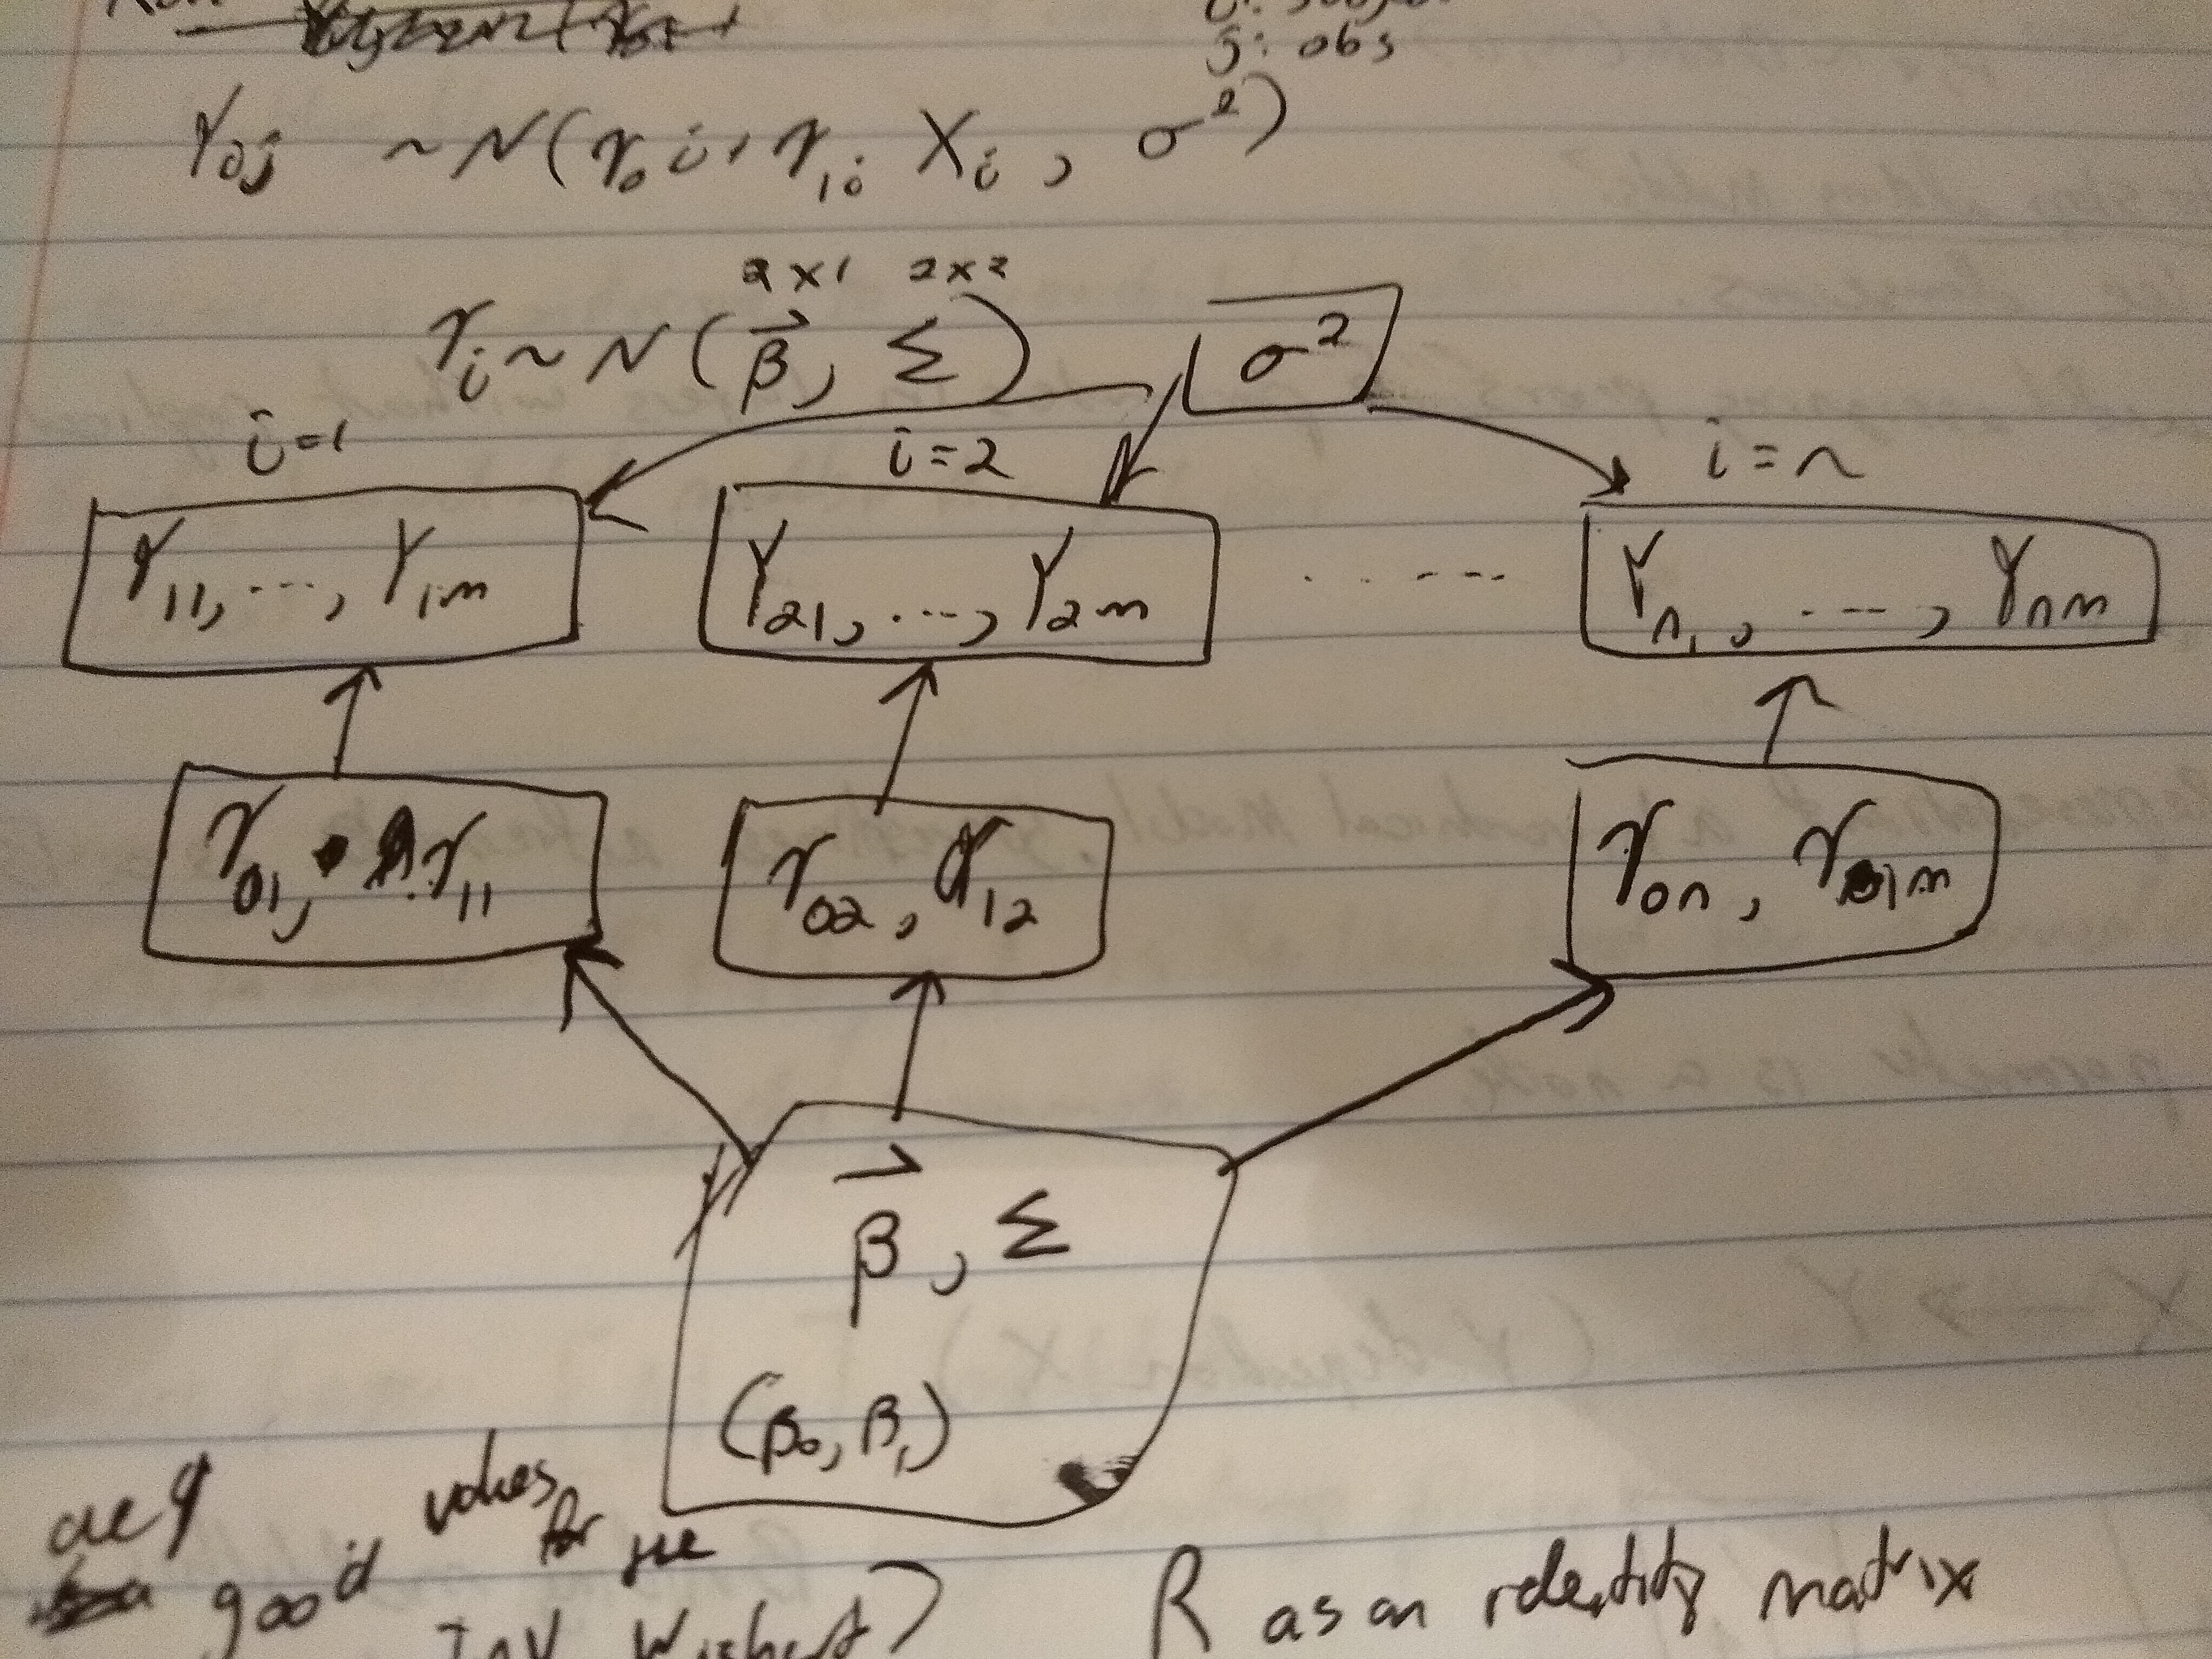
\includegraphics[width=.9\linewidth]{./resources/bdag2.jpg}
\caption{\label{fig:label}Random Slopes Model DAG}
\end{figure}

\begin{quote}
Aside: What are good prior hyperparameters for an Inverse Wishart? It is a subject of much debate. It is thought that choosing R to be an identity matrix is a good idea.  Or choosing K = p + 1 which leads to infinitesimal spread. There isn't generally a \textbf{good} rule of thumb.
\end{quote}

\subsubsection{Missing Data Models}
\label{sec:org00a0d66}

\(Y_i \sim N(\beta_0 + \Sigma \beta_i X_i, \sigma^2)\)


\begin{enumerate}
\item Missing Responses
\label{sec:org5264b0f}

\begin{itemize}
\item Prediction Problem. Can use model to fill in the gaps. What do you think Y might be?
\item Obtain samples from PPD of \(Y_i\)
\item for each MCMC iteration, we draw \(Y_i \sim N(\beta_0 + \Sigma \beta_i X_i, \sigma^2)\). This accounts for random error and uncertainty in the model.
\item If only responses are missing, can we delete them for estimation? No need unless there are patterns in the responses that might be missing. For example, missing temperature data when trying to ascertain whether a heatwave has occurred.
\end{itemize}

\item Missing Covariates
\label{sec:org7cbd6da}
\begin{itemize}
\item Simplest approach is imputation, but doesn't account for uncertainty.
\item MCMC can handle this as well.
\end{itemize}

The main idea is to treat the missing values as unknown parameters. Unknown parameters need priors so missing \(X_i = (X_{i1}, ..., X_{ip})^T\) must have priors \(X_i \sim N(...)\)

If priors are way off, then bad results will be returned.
If specified correctly, lead to inference of \(\beta\)'s in the model.

\textbf{Assumptions about Missing Data}
\begin{itemize}
\item Missing Status is independent of Y and X
\item Covariates are Gaussian
\end{itemize}

There are ways to relax both assumptions but it becomes complicated.

\begin{quote}
If Data are not Missing At Random (MAR), the Bayesian Model will likely give bad results.
\end{quote}

\item Hierarchical LR Model with Missing Data
\label{sec:orga8b4a49}

\(Y_i | X_i, \beta, \sigma^2 \sim N(X_i^T \beta, \sigma^2)\)

\(X_i | \mu, \Sigma \sim N(\mu, \Sigma)\)

\(P(\beta) \propto 1\)

\(\sigma^2 \sim InvGamma(0.01, 0.01)\)
\end{enumerate}

\subsubsection{Closing Thoughts}
\label{sec:orga05a100}

\begin{enumerate}
\item Calibrated Bayes
\label{sec:org93a7324}
\begin{itemize}
\item Mix of Frequentist and Bayesian Approaches
\item Maybe we want a Type 1 error control or 80\% Power.
\end{itemize}

Bayesian is strong for influence under an assumed model, but relatively weak for development and assessment of models. Vice versa for frequentist approaches.

Frequentist approaches for model development and Bayesian methods for inference under a model are ideal in principle. Applied statisticians should be Bayesian in principle.

\item Bayesian Decision Theory
\label{sec:org63bc0e5}
\begin{itemize}
\item Need to determine the ``best'' Bayes method.
\end{itemize}

Should we take posterior mode, median, or mean?

Need a scoring system.

Let \(l(\hat \theta, \theta)\) be a loss function.

\(l(\hat \theta, \theta) = (\hat \theta - \theta)^2\): Squared Loss function (L2 norm?)

\(l(\hat \theta, \theta) = |\hat \theta - \theta|\): Absolute Loss function (L1 Norm?)

Summary of the posterior that minimizes the expected (posterior) loss is Bayes Rule. However, Hypothesis testing requires a more complicated loss function.

\item Bayes Rule for Squared-error loss
\label{sec:orgd1a73c2}

Loss: \(l(\hat \theta, \theta) = (\hat \theta - \theta)^2\)

\(\bar \theta = E(\theta | Y)\): Posterior Mean of \(\theta\)

\textbf{Expected Loss}

\begin{equation}
\begin{split}
E_{\theta | Y} [l(\hat \theta, \theta)] = & E [(\theta \hat - \theta)^2]\\
= & E [(\hat \theta - \bar \theta + \bar \theta - \theta)]\\
= & E [(\theta - \bar \theta)^2 + 2 (\hat \theta - \bar \theta)(\bar \theta - \hat \theta) + (\bar \theta - \hat \theta)^2]\\
= & E [(\theta - \bar \theta)^2] + 2 (\bar \theta - \hat \theta) E[(\hat \theta - \bar \theta)] + (\bar \theta - \hat \theta)^2\\
= & Var(\theta | Y) + (\bar \theta - \hat \theta)^2
\end{split}
\end{equation}

What value of \(\hat \theta\) minimizes \(E [l(\theta, \hat \theta)]\)?

\(\therefore \hat \theta = \bar \theta\) minimizes the expected loss, so \uline{posterior mean} is Bayes Rules

\item Bayes Rule for Hypothesis Testing
\label{sec:orgdb9cdd9}

Let \(\theta = 0\) if \(H_0\) is true. Fail to reject the null hypothesis
Let \(\theta = 1\) if \(H_A\) is true. Reject the null hypothesis.

\(P_0\): Posterior probability of \(H_0\). \(P(\theta = 0 | Y)\).

\(1 - P_0\): Posterior Probability of \(H_A\). \(P(\theta = 1 | Y)\)

$$
l(\theta, \hat \theta) = \begin{cases}
\lambda_1, & \text{Type 1 Error}, \hat \theta = 1, \theta = 0\\
\lambda_2, & \text{Type 2 Error}, \hat \theta = 0, \theta = 1
\end{cases}
$$

If \(\hat \theta = 1\), expected loss function is \(P_0 \lambda_1\)
If \(\hat \theta = 0\), expected loss function is \((1 - P_0) \lambda_2\)

$$
P_0 \lambda_1 < (1 - P_0) \lambda_2 \equiv P_0 < \frac{\lambda_2}{\lambda_1 + \lambda_2}
$$

\item Bias Variance Tradeoff
\label{sec:orgb94b502}

\(Y_i \sim N(\mu, \sigma^2)\)

Estimator 1: \(\hat \mu_1 = \bar Y\)

Estimator 2: \(\hat \mu_2 = c \bar Y\) where \(c = \frac{n}{n + m}\)

\(\hat \mu_2\) is the posterior mean under prior \(\mu \sim N(0, \frac{\sigma^2}{m})\).

Compute the Bias, Variance, MSE of each estimator (MSE = bias\textsuperscript{2} + Var).

Which is preferred?

\textbf{Bias}

\begin{equation}
\begin{split}
E(\mu_1 - \mu) = & E(\bar Y) - \mu\\
= & E(\frac{1}{n} \sum_{1}^{n} Y_i) - \mu\\
= & \frac{1}{n} E(\sum_{1}^{n} Y_i) - \mu\\
= & \frac{1}{n} n \mu - \mu = 0
\end{split}
\end{equation}

\begin{equation}
\begin{split}
E(\mu_2 - \mu) = c E(\bar Y) - \mu = c\mu - \mu = \mu (c - 1)
\end{split}
\end{equation}

As m increases, c becomes less than 1 and will shrink the variance, but more bias will be introduced.

\begin{quote}
In a Bayesian Hypothesis test, \(\lambda_1, \lambda_2\) can be set to control Type 1 error.
\end{quote}

Bayesian estimators have smaller SE because the prior adds information to the model.
Bayesian estimators are biased if prior is not centered on the truth. With a weak prior, the outcomes between a Frequentist approach and a Bayesian Approach are similar.


\item Bayesian CLT
\label{sec:org347ce20}

\textbf{Assumption}
\begin{itemize}
\item Usual MLE conditions on the likelihood.
\item Prior doesn't depend on n and puts non-zero prob on the true value \(\theta_0\).
\end{itemize}

Then

$$
P(\theta | Y) \to N(\theta_0, I(\theta_0)^{-1})
$$

Bayes methods asymptotically unbiased.

Bayes and MLE equivalent with Large Samples but interpretations are different.

Bayes CLT useful for initial values and tuning.

For each regression coefficient, you should have 10x the number of records. When the model is sparse, BLR has much smaller MSE than OLS.
\end{enumerate}
\end{document}
